\documentclass[english,a4paper,twoside]{ppfcmthesis}

\usepackage[utf8]{inputenc}
\usepackage[OT4]{fontenc}
\usepackage{tabularx}
\usepackage{listings}
\usepackage{enumitem}
\usepackage{lmodern}
\usepackage{booktabs}
\usepackage{float}
\usepackage{placeins}
\usepackage{colortbl}
\usepackage{siunitx}
\usepackage{subcaption}
\usepackage{array}
\usepackage{pgfplotstable}
\usepackage{csvsimple}
\usepackage{hyperref}
\usepackage[algoruled]{algorithm2e}
\usepackage{amsmath}
\usepackage{amsthm}
\usepackage{amsfonts}
\usepackage{pdfpages}
\usepackage{xifthen}
\usepackage[export]{adjustbox}[2011/08/13]
\usepackage{grffile}
\usepackage{cleveref}
\usepackage{pdflscape}
\usepackage{rotating}



% DRAFT
\usepackage{draftwatermark}
\SetWatermarkLightness{0.9}
% END DRAFT

\DeclareGraphicsExtensions{.pdf,.png,.jpg}
% \usepackage{tikz}
% \usetikzlibrary{arrows}
\usepackage{ifthen}

\author{
   Amadeusz Juskowiak \album{106453} \and
   Wioletta Różańska \album{106651}}

 \title{Solving quadratic assignment problem --– an algorithm inspired by Physarum polycephalum}

\ppsupervisor{Professor~Jacek~Błażewicz}
\ppyear{2016}

\newlength\longest
\setlist[description]{leftmargin=\parindent,labelindent=\parindent}


\lstset{
  basicstyle=\ttfamily\footnotesize, 
  basewidth={0.5em,0.5em}, 
  frame=single, 
  breaklines=true, 
  language=C++
}

\graphicspath{ {figures/} }

%algorithm2e
\SetAlgorithmName{Pseudocode}{List of pseudocodes}

\begin{document}
\graphicspath{{figures/}}
% Front matter starts here
\frontmatter\pagestyle{empty}%
\maketitle\cleardoublepage%


\includepdf{figures/karta.pdf}
\cleardoublepage

\pagenumbering{gobble}

\chapter*{Acknowledgements}

Foremost, we would like to express our sincere gratefulness to Prof.~Jacek~Błażewicz for his guidance, trust and immense knowledge. His counselling motivated us during research and writing of this thesis.

Besides our supervisor, we are pleased to thank all the members of Laboratory of Algorithm Design and Programming Systems, especially Natalia Szóstak. Without them this thesis would not have come into being. We could not forget about thanking the rest of Poznan~University~of~Technology community. Over the years, their mentoring was an inevitable process which consolidated our life goals. 

Last but not least, we feel the need to express gratitude to our parents, families and friends. They ceaselessly believe in us and their labour formed each of us as the beings capable of expressing themselves.


{
\null\vfill\hfill
\settowidth\longest{\itshape His work is like that of the planter --- for the future. bla bla bla}
\centering
\parbox{\longest}{%
  \raggedright{\itshape%
  The scientific man does not aim
  at an immediate result. He does not
  expect that his advanced ideas
  will be readily taken up. \\
  \vspace{\baselineskip}
  His work is like that of the planter --- for the future. \\ 
  His duty is to lay the foundation for those who are to come, and point the way.\par\bigskip
  }   
  \raggedleft\MakeUppercase{Nikola Tesla}\par%
}
}
\cleardoublepage
\chapter*{Abstract}

The Quadratic Assignment Problem is an optimisation problem with many practical use cases, even though its solutions are usually approximated. It is a representant of NP-hard computation class, therefore there is no algorithm known for solving this problem in polynomial time. Even for a small instances, the computation of the exact assignment can take too much time, which makes it unpractical. This creates a need for various heuristical methods for approximating the solution, which can be used in fields of logistics, computer aided design or even molecular chemistry.

Recently, an emerging computational behaviour of \textit{Physarum polycephalum} is a subject for thorough research. Many works already describe this slime mould as useful in various branches of the computing science. The plasmodial form of \textit{Physarum polycephalum} is used to solve a maze problem, provide a design for a robust network or even approximate the Travelling Salesman Problem. The slime mould is even mathematically modelled and simulated on various levels.

In context of these observations, we transform the gained knowledge of both fields of QAP and \textit{Physarum polycephalum} into an algorithm leading to an approximation of Quadratic Assignment Problem. By observations of a living plasmodium, some of its behaviour is used in a design of the Physarum-based Metaheuristic. This novel method of looking through the search space is used to solve QAP.

As a part of this thesis an implementation of the proposed algorithm is given. It is thoroughfully tested and compared to the already existing methods. It provides useful solutions for many practical use cases, thus proving the suitability for such sophisticated problems. Furthermore, it can be tuned to solve complex instances of QAP or even used for approximating other optimisation problems.
\cleardoublepage

% Table of contents.
\pagenumbering{Roman}\pagestyle{ppfcmthesis}%
\tableofcontents* \cleardoublepage%

% Main content of your thesis starts here.
\mainmatter%

\chapter{Introduction}
\label{chapter:introduction}

Nowadays, computing science intertwines with various fields of studies posing new challenges for the people of the industry. Every aspect of science is dominated by the technology, just like the everyday lives across the world.

A good example of such interdisciplinary connection is a situation when the companies' managers are required to answer a difficult optimisation question. These businesses mostly are made of different branches, which require transferring of goods between them. Each element of the product could be manufactured in a various departments and is needed in the last part of the assembly in the main office. It could be easier when they produce the whole product in one location, yet seldom it is better to divide the responsibility for specialists in each sector. Although, this process generates som extra costs for the company, it would be crucial to minimise the expenses during assignment of the branches to the locations. Trying to resolve this by hand could be a long process due to the complexity of the problem. However, with usage of computers, it could be answered in a shorter time. The result may not be the optimal one in each case, but it should meet most given assumptions, which is enough to put it into real life usage.

In computer science, this dilemma can be stated as the Quadratic Assignment Problem (QAP).  The QAP is a combinatorial optimisation problem, which was defined by Koopmans and Beckmann in 1957 \cite{koopmans-beckmann1957}, and is a generalisation of an assignment problem. It is NP-hard thus even for small instances finding results is done by approximate methods.

The QAP can be formulated as follows: Given $ n $ different facilities ($F$) and $ n $ different locations ($L$), a weight function $ w: F \times F \mapsto R $ between facilities and a distance function $ d: L \times L \mapsto R $ between locations, find the assignment $f$ minimising this cost function:

\begin{equation}
min \sum_{a, b \in F} w(a, b) * d( f(a), f(b))
\end{equation}

Over the years, a number of methods for solving this problem were established. Nevertheless, there is still a place for improvement and experts are searching for new ways of resolving that. Inspired by their works this thesis tries to find an innovative method using living organisms.

The \textit{Physarum polycephalum}, also known as a true slime mould, is a plasmodial organism of yellow colour. Its single cell body is considered to be the biggest in the world \cite{stephenson1994myxomycetes}. Taking into account the current state of classification, it belongs to the Kingdom Protista, however, this used to frequently change due to the fact that it does not exactly match any of the recognised kingdoms. The \textit{Physarum polycephalum} move very slowly, in a branching pattern as it forages for new food sources. It ingests bacteria, fungal spores and during the experiments --- oatmeals.

\section{Motivation}
\label{section:introduction_motivation}

The motivation for this thesis was of our interest not only because of topics related to computing science, but also because of the world around us. The behaviour of \textit{Physarum polycephalum}, which is often compared to a simple machine, creates many opportunities to unveil a biological side of computating science, thus making the topic fascinating.

Nowadays, scientists put great emphasis on discovering and analysing the nature, often improving the world surrounding us. Generally, two ways of development of this field of study could be distinguished. The first one focuses on improving the biological flaws of humans and animals. A good case is a field of studies related to the creation of natural prosthetics, making life easier for the people without limbs. The second one is a transmission of the natural patterns to the computation environment. Observation of nature leads to organic algorithms, usage of which can solve issues seemingly unrelated to initial problem. This can often gives much better results than traditional computer science approach. In example, thanks to such research, the ant algorithm was implemented, which uses the behaviour of an ant colony searching for the best path between their home and food. These unconventional methods of computation provides excellent results for hitherto very complicated mathematical problems.

The slime moulds have a great potential for the algorithmic design in many fields. Until now, several studies linked to these organisms were conducted, though, its computational skills remain a mystery even to experts. One can give an example of the experiment, carried on slime moulds, which solved the maze problem. The organism found the shortest path between two food sources in the environment with walls, thus finding the solution for the maze. More detailed description and more usecases are presented in the following chapter of this thesis. Nonetheless, these interesting achievements were the reason behind the choice of the subject of the thesis

On the other hand, the thesis focuses on the Quadratic Assignment Problem, which is alone a challenging topic. It can be thought as reflecting the real difficulties faced by the managers of logistics companies or electronics designers. They prefer optimal results, however, the complexity of this dilemma makes it almost impossible to find such in a reasonable time. This demand urges scientists to explore this issue further and try to look for a new ways of solving the QAP problem.
The QAP could be a great challenge for inventing a new unconventional algorithm based on the behaviour of physarum.

\section{Goal}
\label{section:introduction_goal}

This thesis presents the road to solving Quadratic Assignment Problem (QAP) based on behaviour of Physarum machines.
Deep analysis of each part of the main dilemma is essential to proceed with future works.

The first task is to carry out the detailed investigation of the behaviour and capabilities of the slime mould. Without the understanding of organisms, it is not possible to replicate its operations. For this purpose, the living plasmodia will be observed, giving us details of the schemes of the movement when looking for food. This will be studied in order to extract similar patterns and facilitate the creation of
calculation method based on them, which could be transported into the computer environment. We will implement such plasmodial behaviour for solving QAP.

Furthermore, not only the direct observation of \textit{Physarum polycephalum} behavior is needed here, but also a careful examination of previous studies. Such research will also give as a thorough look into behaviour and abilities of the slime mould, especially taking into account the possibility of using our model algorithm as an inspiration for solving computational problems.

Next, the analysis of the research related to the QAP in general will be conducted, leading to better understanding of the problem and showing the current practices for solving it. Recognising the dilemma will make it easier to fit the algorithm based on slime moulds to the QAP.

The key element of this thesis is to apply methods used by \textit{Physarum polycephalum} for solving QAP. This step will consist of adaptation of the biological mechanisms, implementation of simulation and analysis of the results. In this way, we connect the previously acquired theoretical knowledge and a practical task. And last, but not least, our aim will be to create the innovative method for solving QAP.

\section{Thesis organisation}
\label{section:introduction_chapters}

The thesis is divided into five chapters and includes three appendices.

\begin{itemize}
  \item Chapter 2 describes the research conducted in order to better understand the problems. It is divided into two parts. The first one describes the \textit{Physarum} organisms characteristics such as a position in the biological classification, basic information about the species, basics of operations, emerging behaviour and previous research. The second part outlines the quadratic assignment problem (QAP). It consists of a different interpretation, practical usages, current exact solution and current heuristic.
  \item Chapter 3 presents an idea for a \textit{Physarum} machine and an algorithm, which are a key part of this thesis. It will be a pseudophysarum machine providing working metaheuristics based on observed behavior.
  \item Chapter 4 describes an implementation of the algorithm and thorougly tests its behaviour and capabilities.
  \item Chapter 5 summarises our research and gives ideas for future work.
  \item Appendix A includes methods of working with a living colony of \textit{Physarum polycephalum}.
  \item Appendix B provides detailed results in tabular form.
  \item Appendix C extends the work with usage of the algorithm for simplified tests for related Travelling Salesman Problem (TSP).
\end{itemize}

\section*{Work Distribution}
\label{section:introduction_distribution}

Both authors wrote the text of this thesis. The rest of the work was distributed between two co-workers in a manner described below:
\begin{itemize}
  \item Amadeusz Juskowiak conducted a research about \textit{Physarum polycephalum} and observed the behaviour of the alive organisms. He also designed and implemented the algorithm approximating QAP.
  \item Wioletta Różańska conducted a research about the quadratic assignment problem. She also implemented the algorithm approximating QAP and carried out comparative tests with existing solutions.
\end{itemize}

\chapter{Background}
\label{chapter:background}

Thorough research of both \textit{Physarum polycephalum} and \textit{Quadratic Assignment Problem} has been conducted. Principles and related works for both fields are presented in following subsections. Obtained knowledge is the ground and an inspiration for a design of solution proposed in a next chapter.


\section{\textit{Physarum polycephalum}}
\label{section:background_physarum}

The organism being a subject for this work is \textit{Physarum polycephalum} also called the many-headed slime mould. It is a member of the \textit{Physaridae} family of slime moulds, in order of \textit{Physarales}, class \textit{Myxogastria}, phylum \textit{Myxomycete}, supergroup \textit{Amoebozoa} in \textit{Protista} kingdom. While current position in taxology is well defined, presented characteristics should justify why scientists used to have problems with classification of the Physarum \cite{stephenson1994myxomycetes}.

In order to make the thesis readable, terms \textit{Physarum polycephalum}, \textit{Physarum} or \textit{the slime mould} will be used interchangeably as the subject is unambiguously defined. As none of the authors have a background in biology, concepts are presented from a computer scientist's perspective in minimal, yet exhaustive, form.


\subsection{Biological characteristics}

\textit{Physarum polycephalum} is a very peculiar organism. Even it is a \textit{Protista}, which are usually very small, it can be observed with a naked eye --- it is one among the biggest currently known unicellular organisms \cite{stephenson1994myxomycetes}. In its natural habitat, under cool, dark and humid conditions the slime mould exists in form of a yellow semistructurised blob (as seen in figure \ref{figure:bp_habitat}). Its occurrence is fairly common around the globe, however species \textit{Physarum polycephalum} does not occur naturally in Poland \cite{narkiewicz2013grzyby}. It feeds on bacteria, fungi and other sources of basic nutrients (such as aminoacids and carbohydrates).

In laboratory conditions, \textit{Physarum} is stored on Petri dishes filled with a non-nutritious agar (figure \ref{figure:bp_petri}). The agar base provides humid environment required for supporting plasmodial stage of the slime mould. A sterile oatmeal or even a soft porridge is used as a controlled source of nutrients. The complete description of a storage and an observation protocol, among other information, is provided in Appendix \ref{chapter:protocol}.

\begin{figure}
  \centering
  \begin{subfigure}{0.45\textwidth}
    \centering
    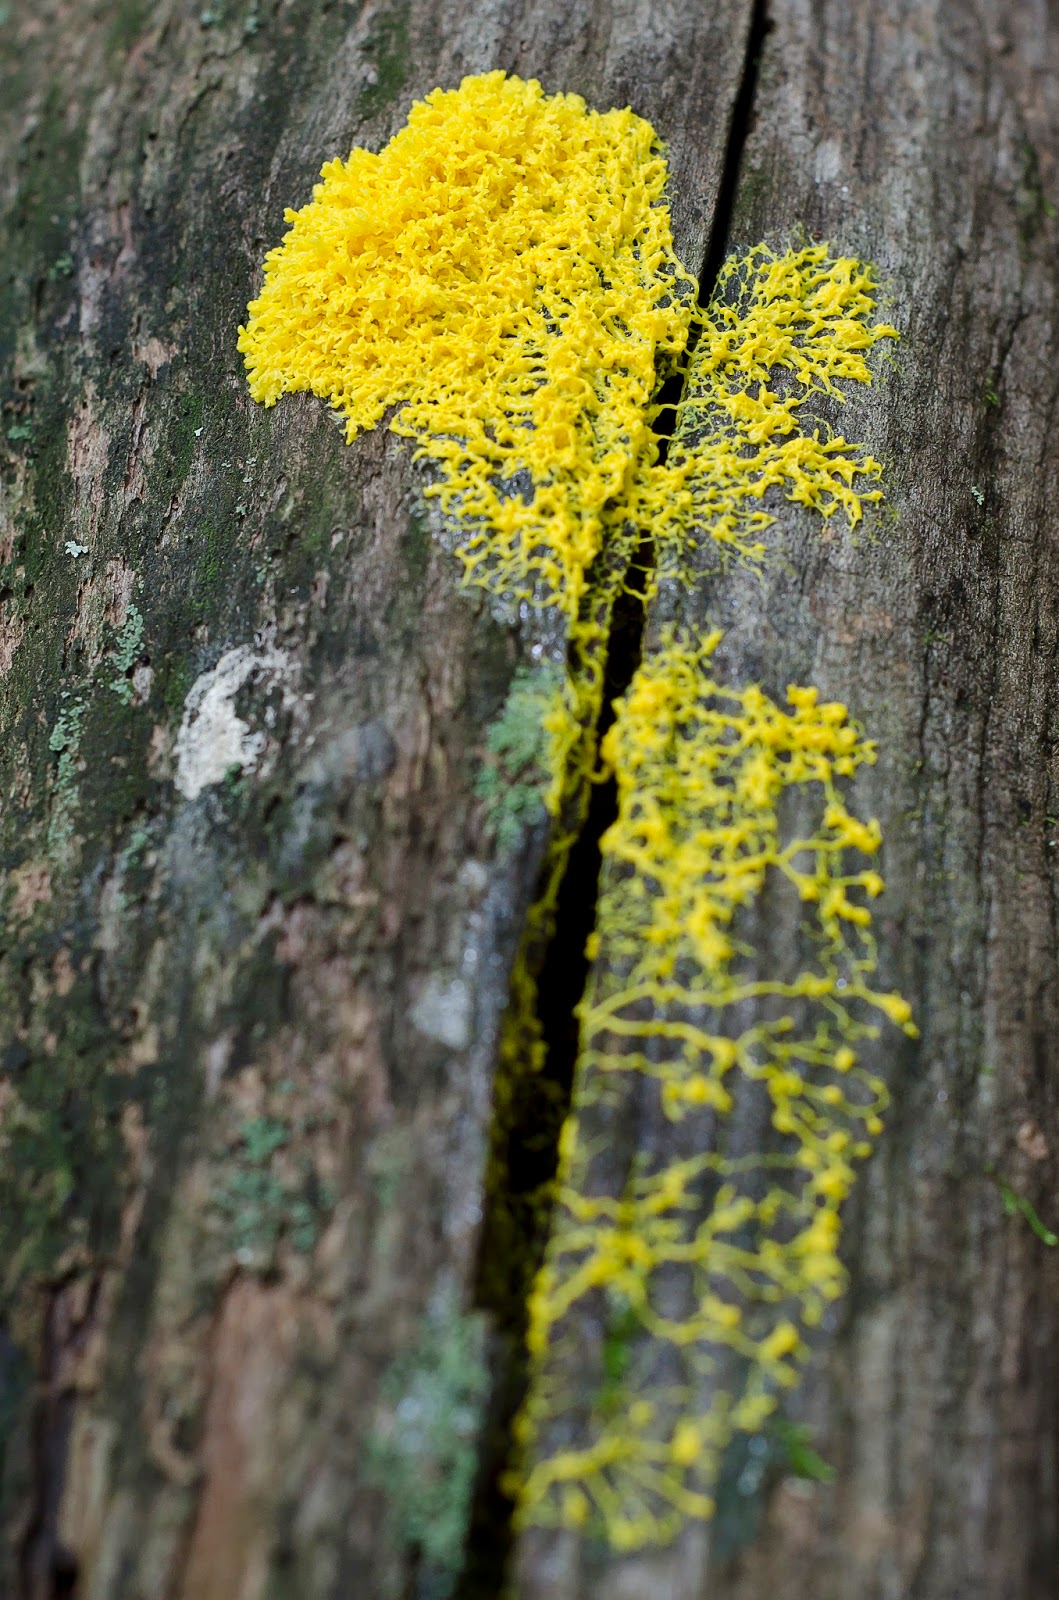
\includegraphics[width=0.9\textwidth]{background/physarum/habitat.jpg}
    \caption{Natural habitat (image source: flickr.com/randomtruth)}
    \label{figure:bp_habitat}
  \end{subfigure}
  \begin{subfigure}{0.45\textwidth}
    \centering
    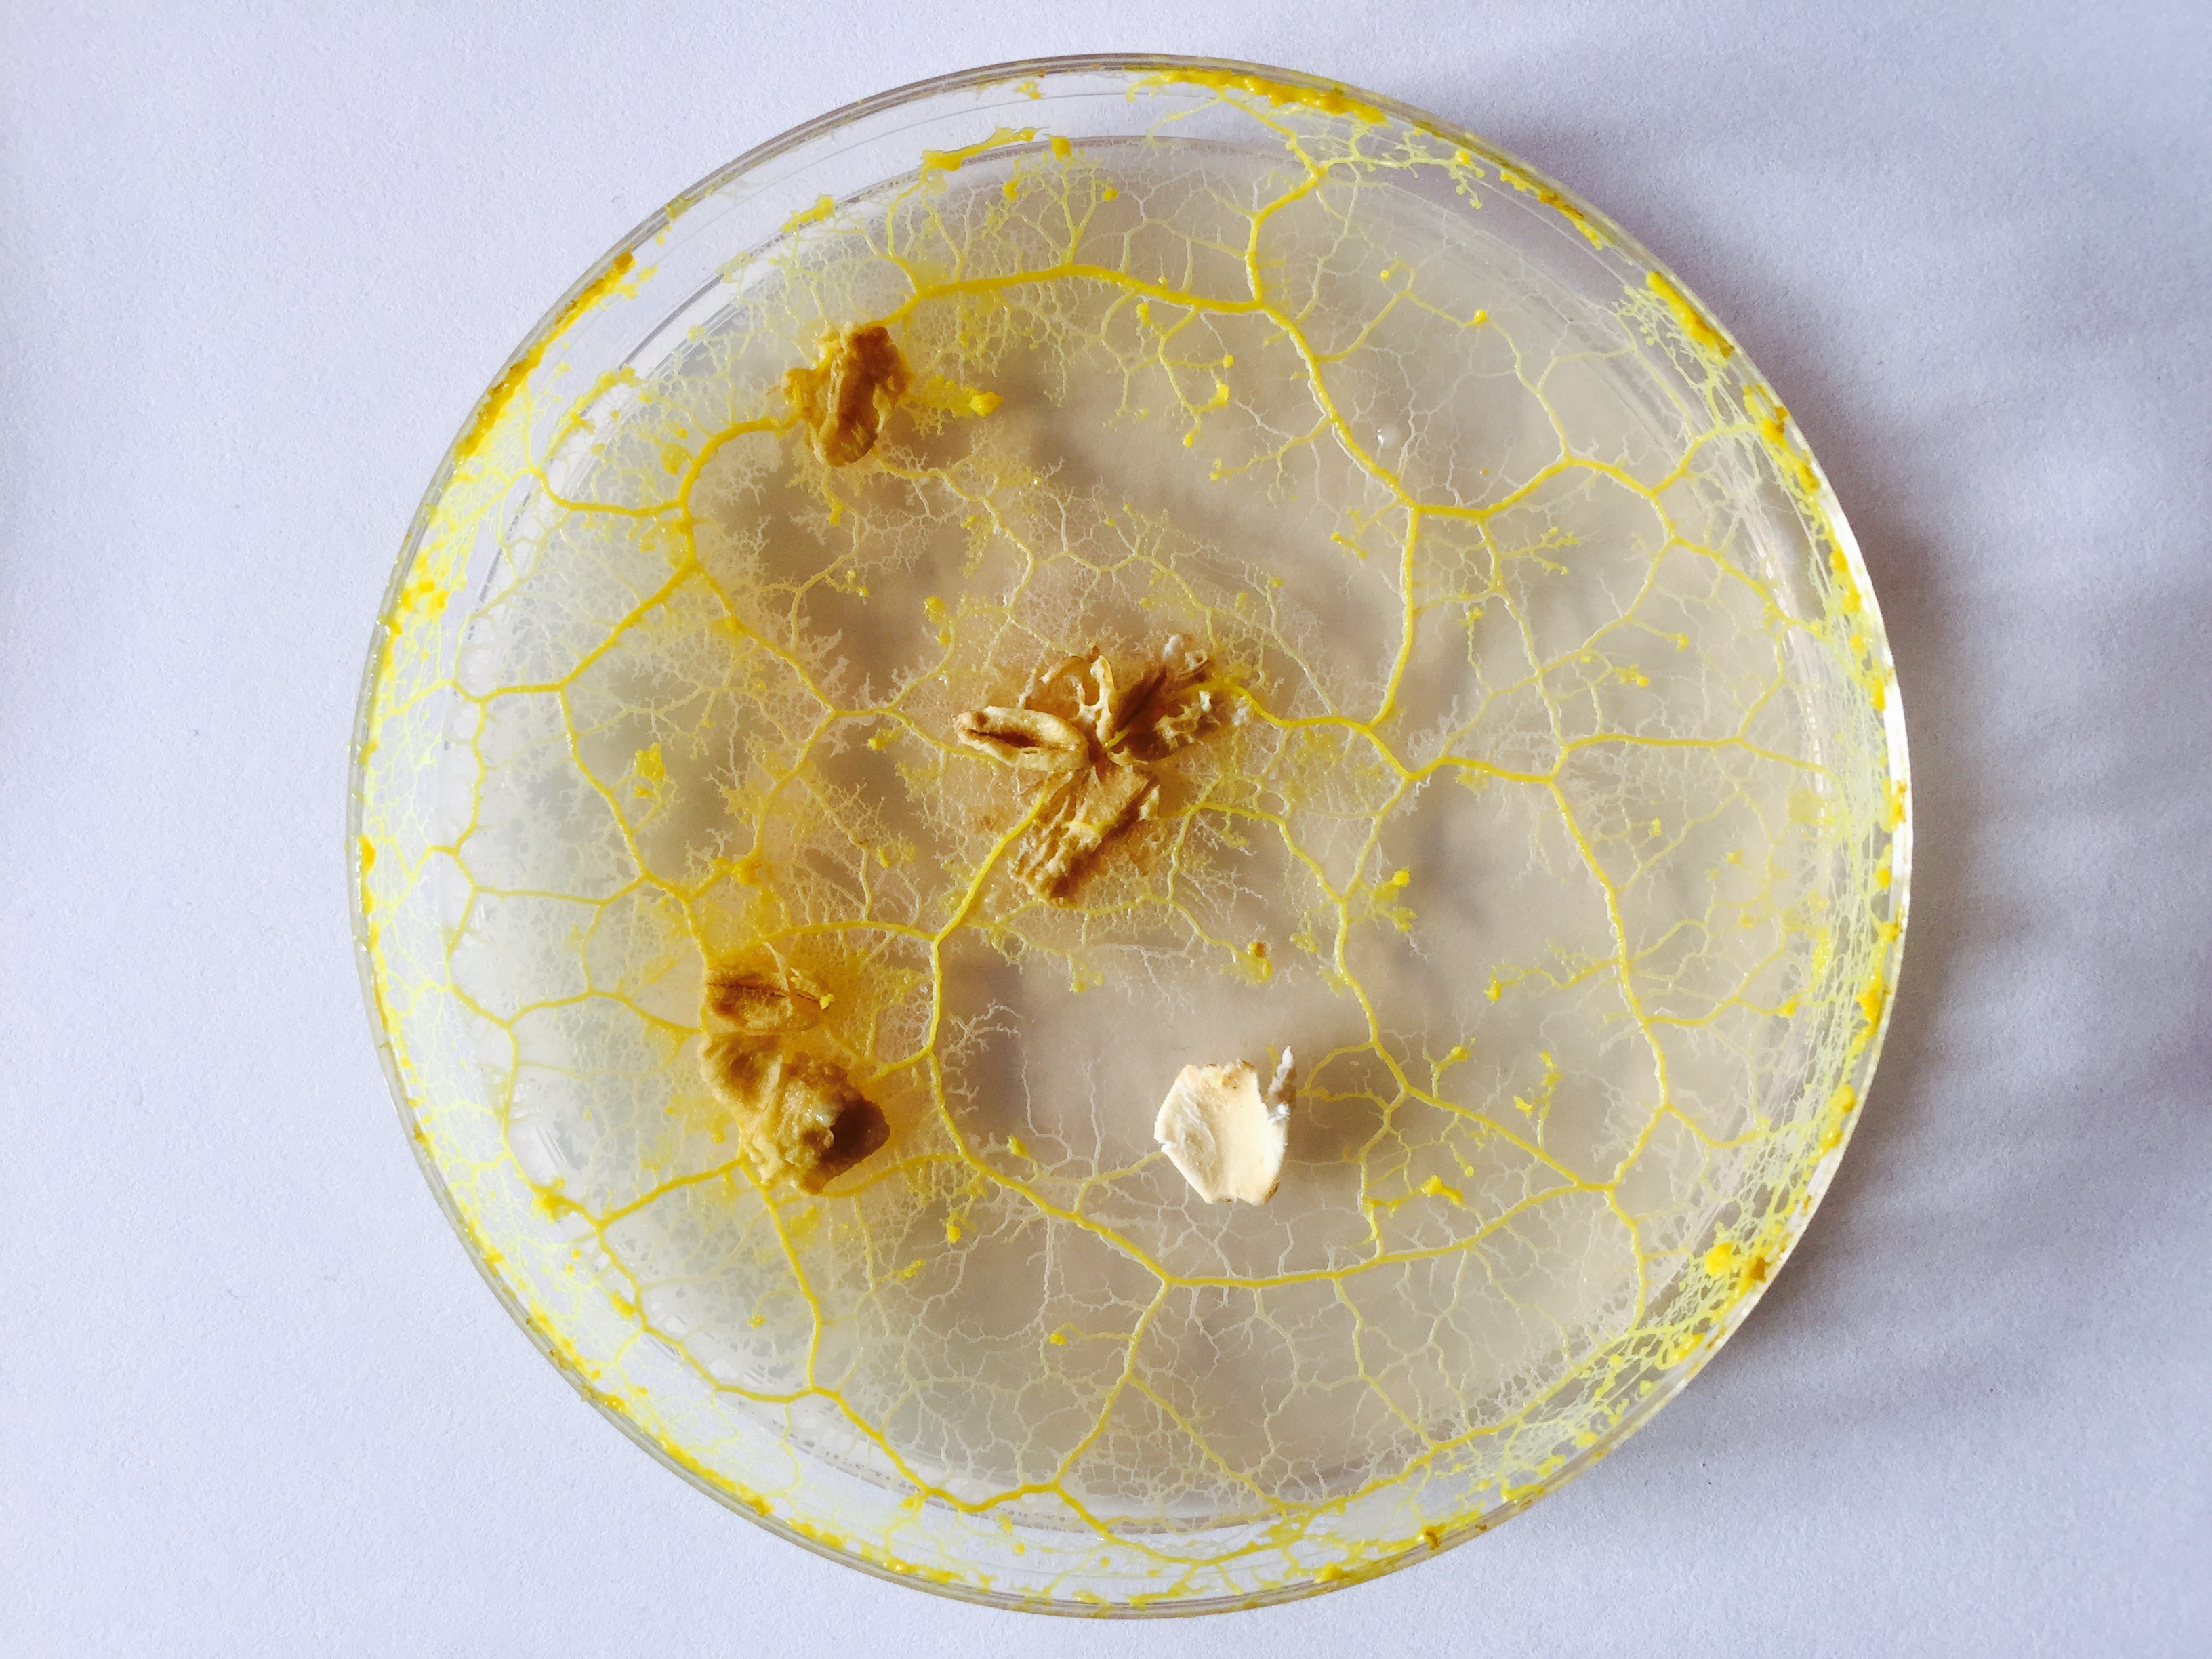
\includegraphics[width=0.9\textwidth]{physarum/IMG_1194.jpg}
    \caption{Petri dish}
    \label{figure:bp_petri}
  \end{subfigure}
  \caption{\textit{Physarum polycephalum} in plasmodial stage}
\end{figure}

\begin{figure}
  \centering
  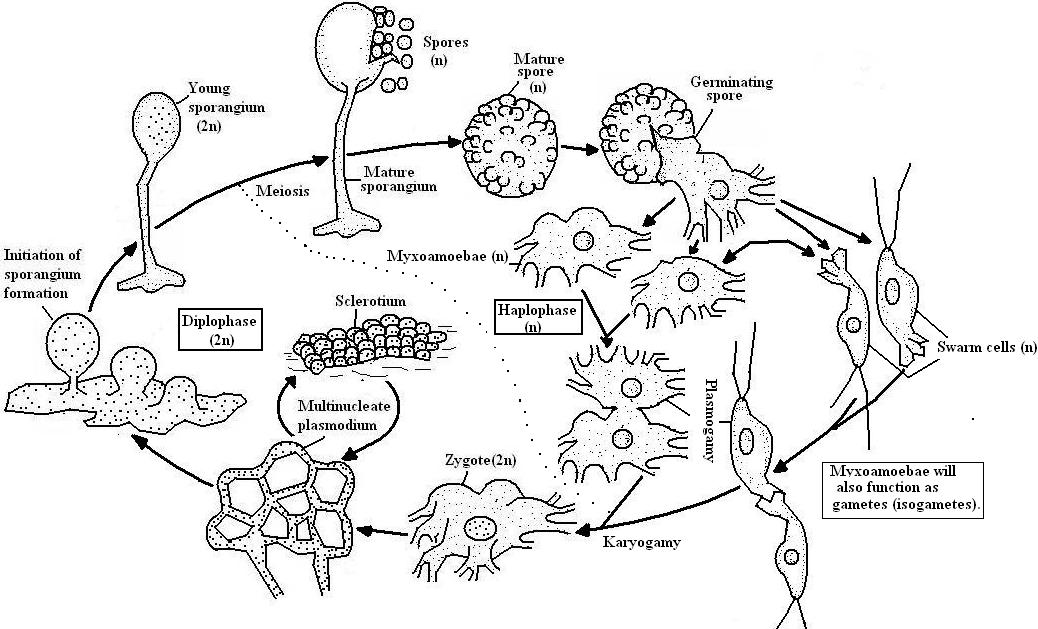
\includegraphics[width=0.94\textwidth]{background/physarum/lifecycle.png}
  \caption{Life cycle of \textit{Physarum polycephalum} (image source: Carolina Biological Supply)}
  \label{figure:bp_lifecycle}
\end{figure}

As representant of \textit{Myxomycete}, a life cycle of the slime mould is very complex, including haploid and diploid phases (as seen in figure \ref{figure:bp_lifecycle}). Such cycle is a result of an evolutionary adaptation \cite{stephenson1994myxomycetes}. Formation of the diploid sporangium occurs as a result of worsening conditions (such as inadequate temperature, humidity or acidity). Sporangium releases spores, which can germinate into ameboid swarm cells. Such cell can enclose into a cyst to protect itself, until environmental conditions improve. When conditions are favourable, the amoeboid cell turns into a flagellated swarm cell. Swarm cells can merge, fuse their nuclei and start mitotic process resulting in a formation of a plasmodium \cite{jones2015pattern}.

For purposes of unconventional computing applications, \textit{Physarum} is preferred in its plasmodial stage. However, during the research transformations into other states are inevitable and must be dealt with. In case of drying or an enforced starvation, sclerotium is formed --- in this dormant phase \textit{Physarum polycephalum} can survive for many years until dampness and nutrients are provided again. Plasmodium forms protoplasmic tubes (also called pseudopodia) as a response to food availability. Such tubes are used for a discovery and transportation of nutrients. The tubes are built in similar way to animal muscles. The ectoplasm contains actin and myosin complexes, which are organised into regular structures that form tubes. Such actomyosin complexes generate a contractile motion which results in streaming of the protoplasm. Furthermore, synchronised oscillations of directions of protoplasm streams can be observed. Nutrients are transported at first in one direction, and after 1-2~minutes the direction is reversed. Period of this oscillation depends on the environment quality and an accessibility of food \cite{wohlfarth1979oscillatory} --- higher frequency oscillations are generated where nutrients are available and favourable environment exist, low frequency oscillations are caused by lack of food or as a result of harmful conditions. 

The plasmodium can grow around 10~mm per hour when it actively explores the environment \cite{coggin1996dynamic}. While moving, plasmodium leaves polysaccharide traces (informally called slime, hence the name slime mould). The network of the protoplasmic tubes adapts, forming efficient ways of transporting nutrients, depending on their amount and quality \cite{nakagaki2004obtaining}. Exploiting this behaviour is a fundamental principle for building physarum machines.


\subsection{Related works}

Since early 1960s \textit{Physarum polycephalum} has been a subject to many biological and microbiological studies \cite{guttes1964mitotic,daniel1962method}, however it is late 70s when its computational-like behaviours have been observed \cite{wohlfarth1979oscillatory}. Research towards computational applications of the \textit{Physarum} truly started in 1990s. Nowadays, there exist two prominent research centres focusing on the slime mould --- one based in United Kingdom (Andrew Adamatzky\footnote{~\url{http://uncomp.uwe.ac.uk/adamatzky/}}, Jeff Jones\footnote{~\url{http://uncomp.uwe.ac.uk/jeff/}} from University of West England, Bristol), second in Japan (Toshiyuki Nakagaki\footnote{~\url{http://www.cris.hokudai.ac.jp/cris/en/research/ob/ob\_innovative/nakagaki.html}}, Hokkaido University, Sapporo). Some of their works excited us about slime mould capabilities and inspired to write this thesis \cite{nakagaki2000intelligence,adamatzky2010physarum,jones2015pattern,adamatzky2007physarum}. Experiments presented here focus on different aspects of \textit{Physarums} behaviour. Understanding them gives impression of emerging computational power of such simple organism as a slime mould.


\subsubsection{Maze-solving capabilities}

Maze-solving or a more constricted problem of finding, preferably shortest, paths is very common in practice. It has many applications and many possible algorithms are already available. Algorithms such as breadth-first search or more complex $A*$ are commonly used for solving mazes \cite{zelkowitz1979principles}. However Toshiyuki Nakagaki et al. proposed usage of slime moulds' natural capabilities as an unconventional solution to this problem \cite{nakagaki2000intelligence}.

In order to use \textit{Physarum} to solve a labyrinth, a maze must be represented as a physical object. Such maze is modelled on a Petri dish where floor is made of non-nutrient agar and walls are made of thin plastic film (the maze used in the experiment is presented on figure \ref{figure:bp_maze_initial}). As the slime mould strictly prefers humid environment of the agar it will not pass arid walls made of plastic film. 

\begin{figure}
  \centering
  \begin{subfigure}{0.45\textwidth}
    \centering
    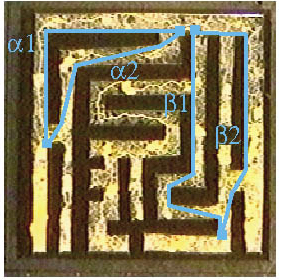
\includegraphics[width=0.9\textwidth]{background/physarum/maze1.jpg}
    \caption{Plasmodium initially filling maze}
    \label{figure:bp_maze_initial}
  \end{subfigure}
  \begin{subfigure}{0.45\textwidth}
    \centering
    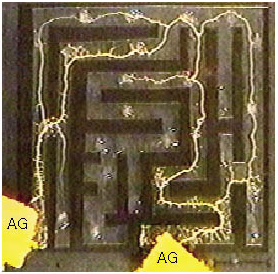
\includegraphics[width=0.9\textwidth]{background/physarum/maze2.jpg}
    \caption{Intermediate state}
    \label{figure:bp_maze_intermediate}
  \end{subfigure}
  \begin{subfigure}{0.45\textwidth}
    \centering
    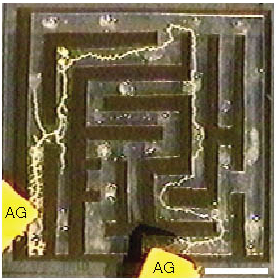
\includegraphics[width=0.9\textwidth]{background/physarum/maze3.jpg}
    \caption{Final route}
    \label{figure:bp_maze_final}
  \end{subfigure}
  \caption{\textit{Physarum} in various states of the maze experiment \cite{nakagaki2000intelligence}}
\end{figure}

There are four possible routes available $\{(\alpha_1,\beta_1), (\alpha_1,\beta_2), (\alpha_2,\beta_1), (\alpha_2,\beta_2)\}$ between entry point $A$ and exit point $B$. The oatmeal-agar-based source of nutrients is planted in both, entry and exit points, while large enough plasmodium is placed over whole floor of the maze. As time passes it can be observed that plasmodium retracts its body from labyrinth's dead-ends, leaving traces of slime where it previously has been placed (figure \ref{figure:bp_maze_intermediate}). 

As a result the slime mould rests only on direct paths connecting the entry with an exit point (figure \ref{figure:bp_maze_final}). Furthermore, it has been observed that \textit{Physarum polycephalum} usually prefers shortest $(\alpha_2,\beta_1)$ path as it prefers most efficient way for transferring nutrients. While obtained results are satisfactory, it must be noted that the whole process takes about 4~hours. 


\subsubsection{Spatial memory}

Memory is usually associated with neurological functions of brain, however it can be externalised in multiple ways, in example as pheromone trails of ants \cite{carroll1973ecology} or even notes-writing as humans do \cite{fisher1973effect}. Team of researchers from University of Sydney, demonstrated that \textit{Physarum polycephalum} uses its slime as a form of spatial externalised memory \cite{reid2012slime}.

A common problem testing autonomous navigational skills in robotics is the U-shaped trap problem \cite{chatterjee2001use}. An efficient solution of this issue requires some kind of a spatial memory or other navigational aids \cite{balch1993avoiding}, therefore it was a good candidate for a test of slime mould's memorising capabilities. The U-maze problem requires an agent (a robot or as in this example the slime mould) to navigate itself from starting position to the goal, where goal is hidden beside the U-shaped trap (figure \ref{figure:bp_trap_model}). The agent has to use some kind of environment map or use a reactive guidance to bypass the trap (figure \ref{figure:bp_trap_model_success}), otherwise, most probably it will be stuck inside the trap (figure \ref{figure:bp_trap_model_failure}).

\begin{figure}
  \centering
  \begin{subfigure}{0.33\textwidth}
    \centering
    \includegraphics[width=0.9\textwidth]{background/physarum/trap_initial.eps}
    \caption{Initial setup}
    \label{figure:bp_trap_model}
  \end{subfigure}
  \begin{subfigure}{0.37\textwidth}
    \centering
    \includegraphics[width=0.9\textwidth]{background/physarum/trap_success.eps}
    \caption{Example successful route to goal}
    \label{figure:bp_trap_model_success}
  \end{subfigure}
  \begin{subfigure}{0.37\textwidth}
    \centering
    \includegraphics[width=0.9\textwidth]{background/physarum/trap_failure.eps}
    \caption{Typical failure}
    \label{figure:bp_trap_model_failure}
  \end{subfigure}
  \caption{U-trap test with possible outcomes}
\end{figure}

The experiment conducted by Reid, Latty, Dussutour and Beekman \cite{reid2012slime} used \textit{Physarum polycephalum} as an agent in the non-nutrient agar environment, where the trap was made out of acetate and the goal was a highly nutritious glucose. The agar base allows diffusion of glucose particles, creating nutrients gradient towards the goal. Initial experiments indicated that \textit{Physarum} moves in a direction where its slime is not present, however if no such direction exists (there is the slime all around plasmodium) it moves in random direction or all over the substrate. Therefore a slime mould has a choice to explore unexplored, however it is not an ultimate one, as it always can maneuver in previously visited areas. 

\begin{figure}
  \centering
  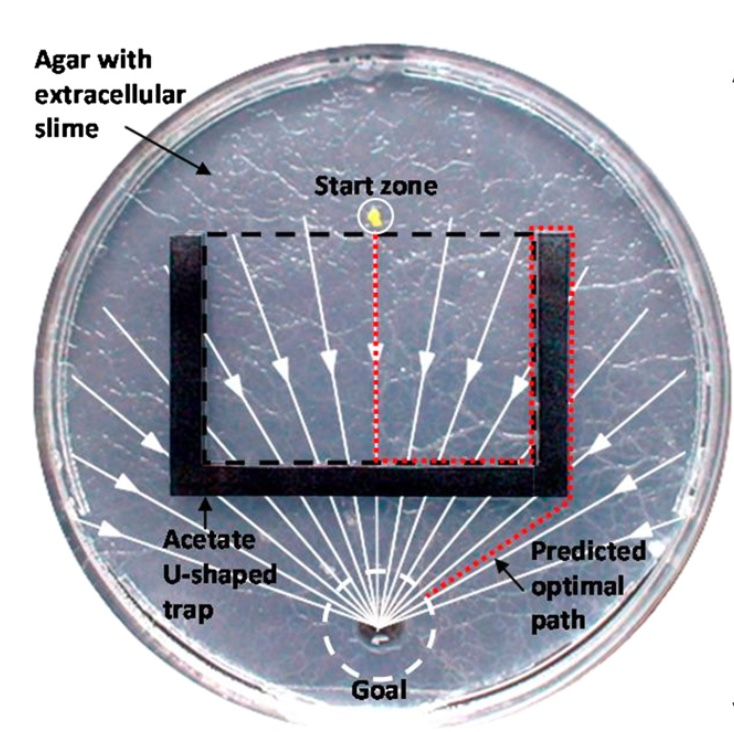
\includegraphics[width=0.74\textwidth]{background/physarum/trap_experiment.jpg}
  \caption{\textit{Physarum polycephalum} in U-trap experiment on a slime covered substrate \cite{reid2012slime}}
  \label{figure:bp_trap_experiment}
\end{figure}

As the slime is a stable nonliving substance, mostly made of galactose polymers it can be easily handled, collected and replanted \cite{mccormick1970isolation}. Two kinds of the experiment have been designed --- in a first one, previously collected slime is placed all over the substrate (figure \ref{figure:bp_trap_experiment}), while in a second one the substrate is just a clean agar. The first environment constrains \textit{Physarum} not to rely on slime for navigation (as implanted slime acts as noise), unlike the second one, in which \textit{Physarum} can use the slime freely for its navigation.

Experiments have shown that \textit{Physarum} placed on a substrate already coated with the slime cannot easily escape out of the U-trap --- it spends there a long time until it leaves the trap. Furthermore, only in 33\% of 24 repeated cases plasmodium reaches the goal. However, when plasmodium is put on a clean agar substrate, an ability to use its slime as the navigational aid results in reaching the goal in 96\% of cases. Both, travelled distance and time to reach the goal, were much shorter when the organism were able to use the slime. These findings prove that \textit{Physarum polycephalum} can sense its extra-cellular slime and uses its existence as a form of an externalised spatial memory for a recognition of previously explored areas.


\subsubsection{Adaptive network design}

Networks are used in a various fields of engineering --- from civil roads, water pipelines, railway systems to energy grids, not to mention the Internet. Design of a practical robust network usually implies a balance between efficiency, cost and fault tolerance. Increasing robustness involves a creation of redundant connections between some of the nodes. This might seem not to be profitable, however it allows the network to gracefully degrade and still maintain some of its throughput. Japanese team of scientists showed that \textit{Physarum polycephalum} can be used to design networks on a par with human or algorithmic designs \cite{tero2010rules}.

% TODO remove letters from pictures
\begin{figure}
  \centering
  \begin{subfigure}{0.33\textwidth}
    \centering
    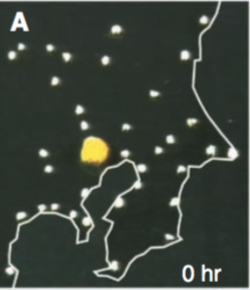
\includegraphics[width=0.9\textwidth]{background/physarum/network_initial.jpg}
    \caption{Initial placement}
    \label{figure:bp_network_initial}
  \end{subfigure}
  \begin{subfigure}{0.33\textwidth}
    \centering
    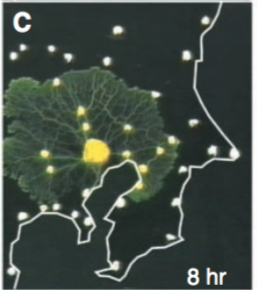
\includegraphics[width=0.9\textwidth]{background/physarum/network_intermediate_a.jpg}
    \caption{State in $t=8h$}
    \label{figure:bp_network_intermediate_a}
  \end{subfigure}
  \\
  \begin{subfigure}{0.33\textwidth}
    \centering
    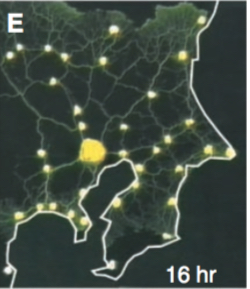
\includegraphics[width=0.9\textwidth]{background/physarum/network_intermediate_b.jpg}
    \caption{State in $t=16h$}
    \label{figure:bp_network_intermediate_b}
  \end{subfigure}
  \begin{subfigure}{0.33\textwidth}
    \centering
    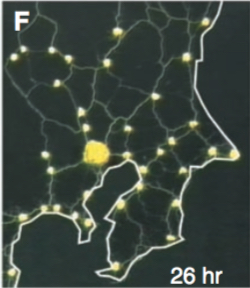
\includegraphics[width=0.9\textwidth]{background/physarum/network_final.jpg}
    \caption{Final plasmodium state}
    \label{figure:bp_network_final}
  \end{subfigure}
  \caption{Example \textit{Physarum polycephalum} network in railway experiment \cite{tero2010rules}}
\end{figure}

The choice of the slime mould was quite natural: the organism forms a network as it forages and it can be assumed, that through many years of evolution, its designs has reached an equilibrium between cost, efficiency and robustness. The researchers prepared an experiment based on design of Tokyo-area rail network. On a substrate made of an agar, thirty~six~food~sources (identical oat meals) have been placed, resembling a real topographical positions of the rail stations (figure \ref{figure:bp_network_initial}). A blob of plasmodium has been placed where city of Tokyo would be, after some time, as the slime mould forages, it covered the substrate and connected each food source (figures \ref{figure:bp_network_intermediate_a}, \ref{figure:bp_network_intermediate_b}). Afterwards \textit{Physarum} retracted its body from the empty areas, leaving only interconnected food sources (figure \ref{figure:bp_network_final}). It should be observed, that some junctions have been left where no food is placed --- these are Steiner~points \cite{kou1981fast} enhancing overall efficiency of the network.

The experiment has been replicated 20~times, each time resulting in slightly different design of the final network, however it always resembled the Tokyo rail network designed by civil engineers. In order to even further improve similarity, the substrate has been illuminated where geographical features restrain the rail network. As the slime mould avoids light, such illumination acted as a constraint for the network --- these networks bore even bigger similarities to original plans than networks made without constraints. 

In the end, it was concluded that networks designed by \textit{Physarum polycephalum} have lower overall cost with similar transport efficiency, however they lack a bit of fault tolerance --- while in only 4\% of faults the real rail network would lead to isolation of any part, in case of networks designed by the slime mould such isolation would occur in 14\% of faults. Still, these results are acceptable as \textit{Physarum}'s network designs have much lower cost. Nonetheless, it should be noted that these networks should not be compared directly --- stops on Tokyo network have not been planned at once, they evolved as the city grew, unlike the task given to \textit{Physarum} which assumed knowledge of stops locations. The processes differs even more, as design of a real rail network is usually centralised, however the slime mould acts as a self-organised mechanism without the central control.


\subsubsection{Slime mould models}

In the same work \cite{tero2010rules}, Japanese researchers proposed a mathematical model of \textit{Physarum polycephalum} used for adaptive network designs based on a flow network. The slime mould has been adapted as initially random lattice, where edges represents the pseudopodia. The flux inside pseudopodia has been accurately defined with Hagen-Poiseuille formula for the laminar flow \cite{sutera1993history}. The simulation is conducted in discrete time steps. In each step a random food source node is selected to drive the flow through the network, where another food source is selected to be a sink. Strength of the flow influences conductivity of each tube --- unused tubes gradually disappear, while effective tubes adapt to increase throughput. This model reflects some of the properties of the real slime mould and can be used for design of adaptive network model.

Quite profound work on modelling \textit{Physarum polycephalum} has been presented by Jeff Jones in his book \cite{jones2015pattern}. He modelled plasmodium in a multi-agent fashion as a material made of multiple particles working towards a reaction-diffusion process. A single agent represents a particle of plasmodium gel/sol structure --- its movement resembles protoplasmic flow, however when it is immobile, it could be treated as the gel matrix. Each agent can sense chemoattractants in the two-dimensional substrate using three forward-directed sensors. A single agent can move in oscillatory or non-oscillatory modes. First one can be used to approximate resistance within plasmodium and the second one represents an ideal movement without any external forces. Plasmodium-like behaviour emerges from the collection of such randomly placed agents. Furthermore chemoattractants and chemorepellents can be placed on the substrate, stimulating the agents to regroup and move. This model can be tuned to closely resemble real \textit{Physarum polycephalum} in a variety of environment conditions.

% TODO crop images so they are aligned
\begin{figure}
  \centering
  \begin{subfigure}{0.3\textwidth}
    \centering
    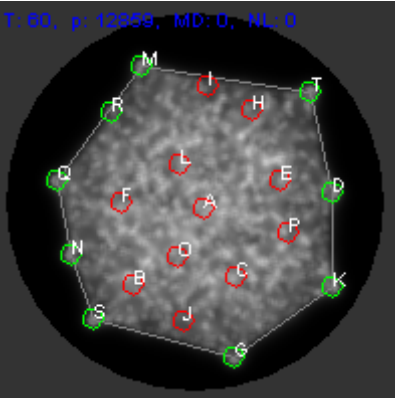
\includegraphics[width=0.9\textwidth]{background/physarum/tsp_initial.png}
    \caption{Initial placement within convex hull}
    \label{figure:bp_tsp_initial}
  \end{subfigure}
  \begin{subfigure}{0.3\textwidth}
    \centering
    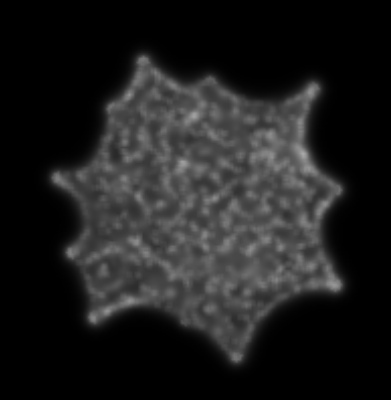
\includegraphics[width=0.9\textwidth]{background/physarum/tsp_intermediate.png}
    \caption{State after removal of some agents}
    \label{figure:bp_tsp_intermediate}
  \end{subfigure}
  \begin{subfigure}{0.3\textwidth}
    \centering
    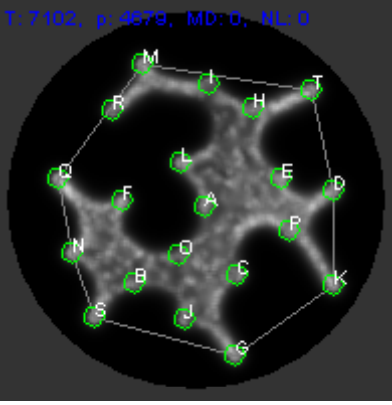
\includegraphics[width=0.9\textwidth]{background/physarum/tsp_final.png}
    \caption{Final state of simulation}
    \label{figure:bp_tsp_final}
  \end{subfigure}
  \caption{Solving TSP using shrinking blob method \cite{jones2014computation}}
\end{figure}

\begin{figure}
  \centering
  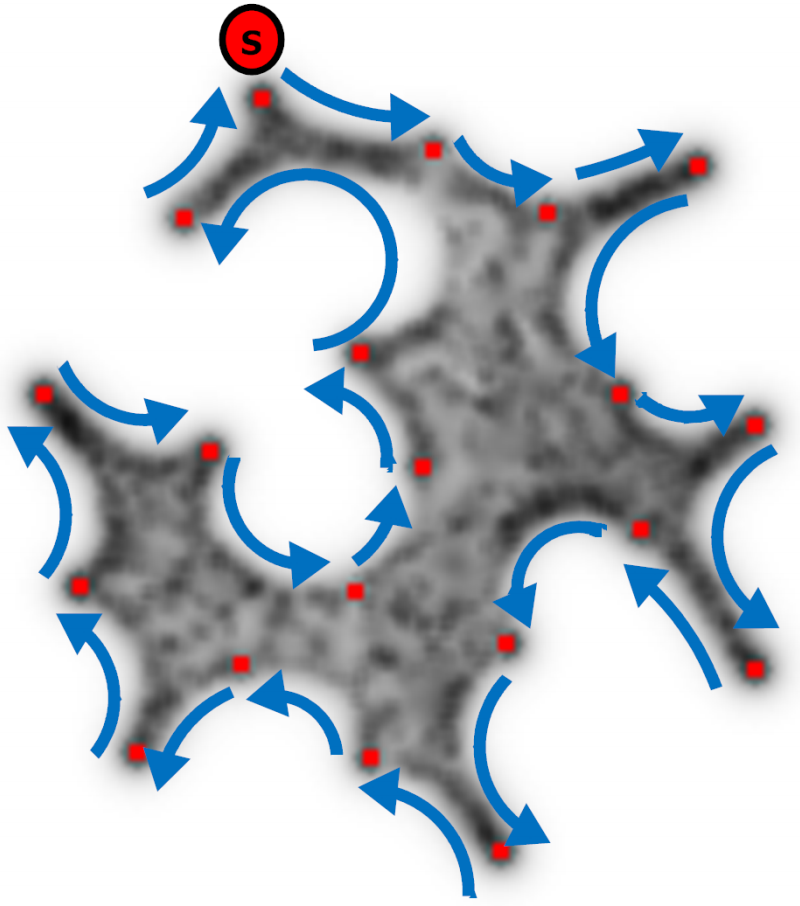
\includegraphics[width=0.3\textwidth]{background/physarum/tsp_readout.png}
  \caption{TSP tour readout method \cite{jones2014computation}}
  \label{figure:bp_tsp_readout}
\end{figure}

Based on this model Jeff Jones and Andy Adamatzky proposed a method of a shrinking blob for approximating solution of Travelling Salesman Problem (TSP) \cite{jones2014computation}. This method requires putting previously described agents inside a convex hull computed on topology of TSP input (figure \ref{figure:bp_tsp_initial}). Initially chemoattractants are placed nearby data points. As simulation goes some agents are removed from the virtual plasmodium, effectively shrinking the blob (figure \ref{figure:bp_tsp_intermediate}). Simulation is stopped when each node is partially uncovered --- a $5 \times 5$ window passes over each node and checks for such condition (figure \ref{figure:bp_tsp_final}). Resulting TSP tour can be read by tracking perimeter of the blob at the end of simulation (figure \ref{figure:bp_tsp_readout}). The authors evaluated this method to be 4.27\% worse than the optimal solutions in their dataset.


\subsection{Observations}

Using the financial support from Poznan University of Technology, we obtained the culture of \textit{Physarum polycephalum} from Carolina Biological Supply. The access to the living organism allowed us to observe its behaviour in a variety of conditions. As for computer scientists, who have no experience in wet lab works, it was a very challenging task to handle alive slime mould, yet very educative one --- detailed methods of handling the organism are presented in Appendix \ref{chapter:protocol}.

We usually worked with the slime mould on a 2\% non-nutrient agar substrate, however two other substrates have been tested: a wet towel and an aluminium foil. We have placed plasmodium on dampened kitchen towel, as we believed that it is easier to manage than the agar solution. As for the wet towel, no mobility has been affected, however water evaporated quickly and regular moisturising has been required. Furthermore moving the colony out of the kitchen towel was more complicated, as it was difficult to cleanly separate the organism from the substrate. In the case of aluminium foil as the substrate, while it makes the separation easy it was not used for long, as this substrate lacks ability to bound water, which is required for keeping \textit{Physarum polycephalum} in its plasmodial stage. A standard non-nutrient agar keeps moisture for a long time (up to 10 days until the plasmodium is moved to new substrate) and keeps smooth surface if properly poured into Petri dish, making it quite easy to relocate the colony. Agar gel-like structure prohibits \textit{Physarum} from escapades to the bottom part of Petri dish, unlike porous kitchen towel. 

We used a classic oatmeal as primary food for the slime mould. It is composed primarily of starch, some proteins, little fat and trace amount of sugar. We usually used oats as a whole or smaller distinct pieces, but for better precision a sterile porridge paste has been used. Nutrients available in oatmeal made the plasmodium move with 9--10~mm/hr (measured on frontier). We experimented with use of table sugar as nutrient, resulting in 8~mm/hr velocity and decolorisation of the plasmodium. Usage of syrup made of pure glucose made the subject to move relatively fast 12--16~mm/hr, however it was completely decolorised and no networking behaviour was observed. It is possible that glucose has dissolved within an agar substrate changing the slime mould's foraging strategy to the simpler one --- no need to look for food as the substrate became source of nutrients. We also confirmed that valerian drops made from valerian root act as strong chemoattractant for the slime mould \cite{adamatzky2012physarum} --- given choice of oatmeal and oatmeal mixed with valerian drops \textit{Physarum} foraged towards the second one in ten of ten cases. Additionally, when multiple sources of food, varying in their size, were introduced to a slime mould, it always ended up foraging on the largest one. In the end we reaffirmed that oatmeals are preferred source of nutrients for laboratory use. As for water, distilled water was used, however when no access to such pure water was possible a tap water has been used. We observed that tap water slightly decreased \textit{Physarum} mobility to abound 8-9~mm/hr, with no other consequences --- it could be caused by chlorine or fluorine used for tap water disinfection \cite{uden1983chlorinated}.

The culture of \textit{Physarum polycephalum} has been kept in dark shoebox as these conditions are favourable for growth of plasmodium \cite{adamatzky2010physarum}. When the slime mould has been kept in a window-lit room, plasmodium growth has been massively reduced (none to as little as 4~mm/hr). However we found that infrared light (near-IR LED has been used) made no observable effects on the plasmodium --- one can use infrared light and infrared camera to observe plasmodium as it forages in the dark. We assume that infrared light carries so little energy, so it makes no harm to the organism. When the Petri dish has been partly lit with visible light \textit{Physarum} strongly avoided bright areas --- it stayed at most 5~mm close to the light patch (as some light has been diffused within agar substrate). A green laser (20~mW power, 520~nm wavelength) has been used with similar results, however the area was lit more precisely. 

Pattern of light can be used to create constraints for the plasmodium --- arrangement of LEDs or lasers can be used for precise limits, some even propose usage of gobo lights or projectors for complex patterns \cite{zhu2013amoeba}. Constraints can be also made using physical or chemical methods. We tested table salt and easily obtainable citric acid as potential chemorepellents. A line made of table salt became an obstacle for crawling plasmodium, it never crossed this line, instead the slime mould bypassed around such obstacle. Same effects have been observed with the citric acid crystals, furthermore enclosing the slime mould within a circle made of citric acid effectively reduced its foraging area to within the circle. While chemical repellents are effective, in a longer term they dissolve into agar substrate, contaminating it and making it unsuitable for keeping the subject alive. Physical based obstacles can be a solution to this problem. We tested two solutions --- removal of agar substrate and addition of thin plastic sheet. Both methods exploit the fact that \textit{Physarum} requires a wet substrate to keep its active plasmodial stage, thus it avoids dry areas. The first method requires cutting out some of the agar resulting in exposing dry area of the Petri dish, where the second one requires cutting pieces of plastic (we used thin yet hard polypropylene foil) and putting them on a top of the substrate creating a dry area. Both methods are \textit{de facto} effective, however we observed unlikely cases (2 out of 10 experiments) where plasmodium has crossed such physical barrier. This observation can be compared to behaviour of an electrical current, which follows path of least resistance, but if insulator is not thick enough it actually can be bypassed --- indeed, usage of thicker physical barriers makes them more robust. 

Hereafter we can conclude that creating barriers is a tradeoff between side~effects and complexity:
\begin{itemize}
  \item light-based --- have no side effects, but are complex to create,
  \item chemical --- easy to create, but with catastrophic long-term effect,
  \item physical --- moderate to create, but somehow unreliable, occupying large area.
\end{itemize}

% TODO add image
The slime mould fed with oatmeal on an agar substrate forages in network structure. Individual oatmeals are connected by pseudopodia varying in thickness. Width of protoplasmatic tubes is proportional to nutrients transported with the flux between nodes of the plasmodium. The organism created many nodes where no food have been placed, thus optimising paths for the nutrients. Moreover during experiments with various food sources and barriers, regular changes in width of the tubes have been observed as response to the local environment. The pseudopodia thickness changed up to 20\% over time span of 60-170~seconds --- frequency of such oscillation has been greater near positive stimulus (food source), lower frequencies have been observed in tubes closer to chemorepellents (such as salt). This behaviour can be used as a form of communication between \textit{Physarum} and other devices --- a time-lapse imaging can be used to acquire such reaction and further processing with Fourier transform \cite{bracewell1965fourier} could be used for interpretation of positive and negative feedback from the \textit{Physarum polycephalum}.

Virtually every available research simplifies \textit{Physarum polycephalum} to a two-dimensional being --- every experiment is conducted on a flat Petri dish, pictures are two dimensional etc. However, by accident we have discovered that the slime mould can make three dimensional structures. When it was kept in a Petri dish with lid closed, with plenty of nutrients in form of oatmeal and well humidified air, plasmodium crawled to the lid, later on dripping from the lid to the bottom of the dish. In the end structures resembling stalagnates have been formed, making the slime mould a three dimensional creature. While some may find this observation somehow useful in designing their experiments, it should be noted that an observation of such structures and feeding the organism is complicated, because the structures prevent Petri dish from opening. 


\section{Quadratic Assignment Problem}
\label{section:background_qap}

The Quadratic Assignment Problem (QAP) is an enormous challenge in the combinatorial optimization.
Its history starts with Tjalling Koopmans and Martin Beckmann, who presented a book named \textit{Assignment Problems and the Location of Economic Activities} in 1957 \cite{koopmans-beckmann1957} and since the presentation of the original formulation, there were no dramatic advances in the improvement of solving methods.
They have focused on the allocation of indivisible resources using the assignment of plants to location as an example.
Two problems were considered, first in which the transportation costs between plants could be ignored and second where the costs are included.

Ignoring the prices shows a relatively simple problem.
The task is to assign into pairs two sets of an equal number $n$ of similar elements.
Each assignment has a different score and after choosing all elements, the sum of rates is calculated.
The objective is to achieve the highest result.
Such dilemma is named linear assignment problem.

Companies often have many tasks with different difficulties for their workers.
Each employee could do the task more or less with the likewise result, which will be the rate of the pairing.
Picking the most fitting person for the specific duty could be a valid example of this simplistic problem.
However, this expects that each person is suitable to do the activity alone.
Adding that tasks hinge on each other makes selection less trivial.

Introducing an assumption that some elements from one set are dependent on other elements from the same set complicates greatly linear assignment problem and presents quadratic assignment problem.
In this situation, we have two collections as before and a matrix with weights, where each matrix's element represents one combination of assignment.
Here, choosing the solution for even a small number of elements could be demanding.

The problem's importance could be shown by real life patterns existing in many fields of studies.
In production, assigning different factories to locations is one of them.
Plenty of companies need to divide responsibilities between each facility, so they could create various parts of a product, which would be later assembled together at the main branch.
The factories need to communicate constantly and allow movement of items between them.
Here, the essential factor is the distance.
The most dependent branches should be closer to each other in order to accelerate production.
It fits perfectly the presented dilemma because minimising the total cost of transportation could be achieved only by allocating items smartly.
It also matches the model - there are two sets, locations, and factories, with an equal number of elements and facilities dependent on others.

In electronics, the backboard wiring problem could be an example.
Placement of distinctive elements on the backboard is not a trivial task.
Items contingent on others creating a net connected by wire.
The longer the coil, the resistance is bigger.
This affects the performance of the whole electrical network and minimisation is indicated.

In the service industry, an example could be locating distinct departments.
Similar to factories and location, here, offices and floors or rooms are allocated.

\subsection{Mathematical definition}
The Quadratic Assignment Problem (QAP) can be generally presented as:
\begin{equation}
min \sum_{a, b \in F} w(a, b) * d( f(a), f(b))
\end{equation}

where $w$ is a weight function $w: F \times F \mapsto R$ between $m$ different facilities ($F$) and $d$ is a distance function $d: L \times L \mapsto R$ between $m$ various locations ($L$). $y = f(x)$ means assignment of the facility $x$ to location $y$.

This could be extended to a quadratic integer problem formulation:
Let $m$ be positive integer and $M = { 1, 2, ..., m }$. The Quadratic Assignment Problem (QAP) can be formulated as
\begin{align}
  \text{minimize} &\null \sum_{i \in M} \sum_{j \in M} \sum_{p \in M} \sum_{q \in M} a_{ijpq}x_{ij}x_{pq} + \sum_{i \in M} \sum_{j \in M} b_{ij} x_{ij} \\
  \text{subject to} &\null \sum_{i \in M} x_{ij} = 1, \; j \in M \\
  &\null \sum_{j \in M} x_{ij} = 1, \; i \in M \\
  &\null x_{ij} = 0 \; or \; 1, \; i, j \in M
\end{align}

where $a_{ijpq}$ indicates the ratio of flow between factories $i$ and $p$ and distance between their assigned locations $j = f(i)$ and $q = f(p)$.
The assignment of factory $i$ to location $j$ is symbolised by $x_{ij} = 1$.
Additionally the $b_{ij}$ is the cost of such assignment, which may or may not be taken into consideration depending on the instance of the problem.

This formulation is the most generalised model of quadratic assignment problem.
It could have been defined differently, however, this shows the objective function as a quadratic one, which clearly indicated the name.
The discrete nature and the complexity of quadratic objective function cause difficulties in finding an optimal solution thus making the problem NP-hard.
Horowitz and Sahni have proved in their book \cite{horowitz1978fundamentals} that QAP needs an exponential time algorithm to solve optimally.


\subsection{Known algorithms}
\subsubsection{Exact solutions}

The most simple method of resolving QAP is by using an enumeration, which evaluates all of the $m!$ permutations (assignments) and records the best solution \cite{frazer1997602}.
Every calculation must be done from the start.
This requires $m^2$ steps and must be computed $m!$ times, which makes it useless for bigger instances.
However, when the problem is small, it has an advantage due to simplicity - the implementation is simple and requires little memory.

Surprisingly, also the time could be improved. Franzer presented in his paper \cite{frazer1997602} that for test problem with $m=10$ the enumeration could be faster than linear programming. Comparisions of the memory usage also gave amazing results thus proving that linear or 0-1 programming are not the most efficient, therefore appropriate, solution methods in this case.

\subsubsection{Linearizations}
One approach to resolve a complex problem is to reduce it to a linear programming problem.
Unfortunately, most of the time this could be impractical even for small $m$. Lawler \cite{lawler1963} was the first to transform the problem. He represented it by an equivalent 0-1 linear programming problem and facilities the computations. He based his thinking on a travelling salesman problem looking for similarities between these two \cite{charnsethikul1988exact}.

Defining $m^4$ variables $y_{ijpq}$ as $m^2$ variables $x_{ij}$ where
\begin{equation}
y_{ijpq} = x_{ij}x_{pq}
\end{equation}
the problem can be linearised and stated as
\begin{align}
  \text{minimize} &\null \sum_{i \in M} \sum_{j \in M} \sum_{p \in M} \sum_{q \in M} a_{ijpq}y_{ijpq} + \sum_{i \in M} \sum_{j \in M} b_{ij} x_{ij} \\
  \text{subject to} &\null \sum_{i \in M} x_{ij} = 1, \; j \in M \\
  &\null \sum_{j \in M} x_{ij} = 1, \; i \in M \\
  &\null x_{ij} = 0 \; or \; 1, \; i, j \in M \\
  &\null \sum_{i \in M} \sum_{j \in M} \sum_{p \in M} \sum_{q \in M} y_{ijpq} = m^2 \; \\
  &\null x_{ij} + x_{pq} - 2y_{ijpq} \leq 0, \; i, j, p, q \in M \\
  &\null y_{ijij} = 0 \; or \; 1, \; i, j, p, q \in M \\
\end{align}
As the result there are $m^4 + m^2$ binary variables and $m^4 + 2 m^2 + 1$ constraints. However, Lawler's definition is still impractical for any bigger $m$.

Kaufmann and Broeckx \cite{kaufman1978algorithm} created another linearisation, which has the smallest number of variables and constraints and is based on the method suggested by Glover \cite{gueye2009linearization}.
Such manipulation reduces the complexity of the problem thus making calculations faster.
The authors rearrange the objective function into
\begin{equation}
  \sum_{i \in M} \sum_{j \in M} x_{ij} \sum_{p \in M} \sum_{q \in M} a_{ijpq} x_{pq}
\end{equation}

Afterwards they define $m^2$ new real variables
\begin{equation}
  w_{ij} := x_{ij}\sum_{p \in M} \sum_{q \in M} a_{ijpq} x_{pq}
\end{equation}

Additionally introducing $m^2$ constraints $ c_{ij} := \sum_{p \in M} \sum_{q \in M} a_{ijpq} $ the problem could be formulated as
\begin{align}
  \text{minimize} &\null \sum_{i \in M} \sum_{j \in M} w_{ij}\\
  \text{subject to} &\null \sum_{i \in M} x_{ij} = 1, \; j \in M \\
  &\null \sum_{j \in M} x_{ij} = 1, \; i \in M \\
  &\null x_{ij} = 0 \; or \; 1, \; i, j \in M \\
  &\null c_{ij}x_{ij} + \sum_{p \in M} \sum_{q \in M} a_{ijpq}x_{pq} - w{ij} \geq c_{ij} = 0 \; i, j \in M \\
  &\null w_{ij} \geq 0, \; i, j \in M \\
\end{align}

As the result there are $m^2$ real variables, $m^2$ binary variables and $m^2 + 2m$ constraints.
This improves slightly previous methods.
However, Kaku and Thompson \cite{kaku1986exact} reported that for small sizes, such as m = 8, the requirements become too large and optimality could not be proved.

Another linearisation was presented by Frieze and Yadegar \cite{frieze1983quadratic}.
Obtaining their mixed integer linear programming formulation could be achieved by replacing the product of binary variables by continuous variables as
\begin{equation}
  y_{ijpq} := x_{ij} x_{pq}
\end{equation}

The outcome definition is as follows
\begin{align}
  \text{minimize} &\null \sum_{i \in M} \sum_{j \in M} \sum_{p \in M} \sum_{q \in M} a_{ijpq}y_{ijpq} + \sum_{i \in M} \sum_{j \in M} b_{ij} x_{ij} \\
  \text{subject to} &\null \sum_{i \in M} x_{ij} = 1, \; j \in M \\
  &\null \sum_{j \in M} x_{ij} = 1, \; i \in M \\
  &\null x_{ij} = 0 \; or \; 1, \; i, j \in M \\
  &\null \sum_{i \in M} y_{ijpq} = x_{pq}, \; j, p, q \in M \\
  &\null \sum_{j \in M} y_{ijpq} = x_{pq}, \; i, p, q \in M \\
  &\null \sum_{p \in M} y_{ijpq} = x_{ij}, \; i, j, q \in M \\
  &\null \sum_{q \in M} y_{ijpq}= x_{ij}, \; i, j, p \in M \\
  &\null y_{ijij} = x_{ij}, \; i, j \in M \\
  &\null 1 \geq y_{ijpq} \geq 0, \; i, j, p, q \in M
\end{align}

In this case, there are $m^4$ real variables, $m^2$ binary variables and $m^4 + 4m^3+m^2+2m$ constraints.

Adams and Johnson \cite{adams1994improved} presented also a new 0-1 linear integer programming formulation.
It has similarities to the previous definition.
\begin{align}
  \text{minimize} &\null \sum_{i \in M} \sum_{j \in M} \sum_{p \in M} \sum_{q \in M} a_{ijpq}y_{ijpq} \\
  \text{subject to} &\null \sum_{i \in M} x_{ij} = 1, \; j \in M \\
  &\null \sum_{j \in M} x_{ij} = 1, \; i \in M \\
  &\null x_{ij} = 0 \; or \; 1, \; i, j \in M \\
  &\null \sum_{i \in M} y_{ijpq} = x_{pq}, \; j, p, q \in M \\
  &\null \sum_{j \in M} y_{ijpq} = x_{pq}, \; i, p, q \in M \\
  &\null y_{ijpq} = x_{pqij}, \; i, j, p, q \in M \\
  &\null y_{ijpq} \geq 0, \; i, j, p, q \in M
\end{align}

So we have are $m^2$ binary variables, $m^4$ continuous variables and $m^4+2m^3+2m$ constraints.

\subsubsection{Metaheuristics}
Methods presented previously are not efficient to bigger instances.
In order to enhance the results, heuristics were used.
These approximate solution techniques have been adopted to facility combinatorial problems.
After it became clear that many of dilemmas are NP-hard, the role of heuristics increased.
Even though problems of dimensions $m > 20$ are still impractical to resolve due to high computational time, heuristics slightly improved a situation for medium size cases.

\paragraph{Greedy}

The easiest heuristic is a greedy algorithm.
In each step, a choice is made trying to locally improve at the current solution.
After a while, when the algorithm does not see a chance to improve, it stops.
The biggest disadvantage of this approach is that it may never reach global optimum due to locking in a local one. A type of such method is a steepest algorithm, where the next result is the best neighbour.


\paragraph{Genetic algorithm}

A genetic algorithm (GA) is inspired by the processes of natural selection.
It uses the analogies from a real world such as mutation, crossover and selection occurring in biology and belongs to the class of evolutionary algorithms (EA).
Its high-quality solutions make it commonly utilised.
The first genetic algorithm was presented by Holland \cite{holland1975adaptation} in 1975.

At the beginning, there is a set of initial feasible solutions, which are generated randomly.
This is called the \textit{initial population}.
An \textit{individual} is usually an element of the initial population.
From the current group, the algorithm selects a number of \textit{parents}, which are pairs of individuals.
Each pair of the parents is used to create a new feasible solution, \textit{child}, using \textit{cross-over rules}.
In the situation that the child solution is corrupted, it needs to be thrown out of the current population.
Until fulfilment of \textit{stop criterion}, which examples are run-time, a specific number of operation etc, these steps are continued.
Periodically, \textit{mutations} or \textit{immigrants} are applied to population.
They diversify the genes by modification of current individuals or replacement of them so that the overall quality of future results could be improved.

QAP has been tested with such genetic algorithm.
The first one, presented by Tate and Smith \cite{tate1995genetic}, did not achieve great results - for the small size of instances, it struggled to provide the optimal solution.

Even though it seemed that GA did not suit property for QAP, hybrid approaches showed otherwise.
They introduced local optimization tools by using \textit{tournaments}.
During the tournament, several runs of GA are initialised from different initial populations.
After stopping them, a new population is derived as a union of all the runs.
Next, the new population is given as an initial population to a new run of GA.
A good example was presented by Ahuja, Orlin, and Tiwari \cite{ahuja2000greedy} presented in 1995, which gave excellent results comparing to classical GA.

\paragraph{Tabu search}

In the beginning of heuristics, the most popular approach was Local Search.
Starting from one solution, the algorithm was improving it by applying slight modifications.
Tabu search is a metaheuristic local search method created by Glover \cite{glover1986future} in 1986, which improves the problems encountered in Local Search.
Its goal is to conquer local optimality using not only advancing the result, but also worsening.
It is achieved by remembering already visited outcomes, which helps to see promising directions for further exploration.
This approach shows the best results for QAP.

The method has few main elements, which needs to be defined in order to understand the procedure:
\begin{itemize}
  \item A \textit{search space} is a space of all possible solutions that could be visited during the search. This includes all feasible answers of the problem.
  \item A \textit{neighbourhood structure} is a subset of search space, which could be achiveved by applying a single \textit{transformation} to a current solution.
  \item A \textit{move} is an operation, which changes solution $x$ to a neighbour $x'$. In the case of QAP, the neighbourhood could be created by exchanging one pair of the solution.
  \item A \textit{tabu list} is a list containing forbidden (tabu) moves and it is updated constantly with each iteration. It consists of the records of the recent history of transformations and prevents cycling back to already visited result.
  \item An \textit{aspiration criterion} is a condition associated with each tabu move, which permits cancelling its tabu state. A most common example is allowing the tabu move if the value of the objective function is superior to current. This means that the solution was not previously visited.
\end{itemize}

At the beginning, the feasible solution is chosen and the tabu list is updated.
There is also a list of neighbours available.
The algorithm chooses the best neighbouring solution, which could be produced by a non-tabu move.
The neighbour does not have to raise the value of objective function.
Afterwards, the neighbour is the current result and the algorithm goes from the start.
The calculations are ended after \textit{termination criteria}, which could be either fixed number of iterations or the number of iterations without an improvement in the value, after reaching the threshold value.

In order to prevent visiting the same solutions over and over, a tabu criterion is used.
It identifies moves, which could lead to cycles, and adds them to the tabu list.
However, such moves could be applied if the aspiration criterion shows that they could introduce potentially winning solutions.
The tabu list is an essential change comparing to the local search.

Each tabu search algorithm could be implemented slightly differently, which impede measurement of performance.
Currently, three different tabu search methods were proposed.
First, a fixed tabu list proposed by Skorin-Kapov \cite{skorin1990tabu}.
The size of tabu list is a parameter, which needs to be tuned before starting the calculation.
It can also be dependent on the specific instance, thus such method is not recommended.
Second, a robust tabu search proposed by Taillard \cite{taillard1991robust}.
Here, a maximum and a minimum are defined and the size of the tabu list is chosen among them.
Third, a reactive tabu search proposed by Battiti and Tecchiolli \cite{battiti1994reactive}.
The size of the tabu list is adapting to the current situation.
When the cycle is identified, the size is increased according to the length of the repetition.

\paragraph{Simulated annealing}

Simulated annealing (SA) is a heuristic which searches locally a big exploration space.
The method, firstly presented by Kirkpatrick, Gelatt and Vecchi \cite{kirkpatrick1983optimization} and {\v{C}}ern{\`y} \cite{vcerny1985thermodynamical}, is based on the analogy to annealing known from metallurgy.

The first step includes generating the initial feasible solution and calculating its value using the cost function.
After that, the neighbouring result is produced and its rate estimated.
Both of them are compared, and if the cost of the neighbour is smaller than current solution then the algorithm moves to the neighbour.
Otherwise, it may move to the new solution.
The decision is made by determining \textit{acceptance probability} and opposing it to a random number.
This helps to avoid local optima.
These steps are repeated until a satisfactory solution is found or the specified number of iterations are reached.

A very important element is the acceptance probability function.
Taking into account the new cost, the old cost and the current temperature it calculates a number between 0 and 1.
The result is a guidance whether to switch solution or not.
This cost is compared with a randomly generated number from the same range.
If the acceptance probability is larger than the second number then the new current solution is the neighbour.

The temperature is another element of the algorithm.
It starts at 1.0 symbolising heat and that all particles are randomly arranged in this liquid state.
With each iteration it is multiplied by a constant typically between 0.8 and 0.99 and as the temperature decreases the probability tends to concentrate on low energy states.
This slightly decreases the value and simulates slow cooling of the metal.
It is also used as a stopping criterion - algorithm stops when the temperature reach 0.
At the end, at thermal equilibrium, the probability that a system is in a configuration $i$ with energy $E_i$ is given by Boltzmann distribution:

\begin{equation}
  p_i = \frac{exp(-\frac{E_i}{kT})}{S}
\end{equation}

Here $T$ is the absolute temperature, $k$ the Boltzmann constant, $N$ the total number of configurations and
\begin{equation}
  \sum_{i=1}^{N} p_i = 1
\end{equation}

Burkard and Rendl \cite{burkard1984thermodynamically} have applied SA to the QAP.
They have presented that if the problem could have a neighbourhood defined, it can be solved using SA, thus this algorithm is a general heuristic.
Other authors presenting SA to solve QAP are Wilhelm and Ward \cite{wilhelm1987solving} and Connolly \cite{connolly1990improved}.
Each of them defined neighbour as a solution with one pair-exchange from the current.
The difference between them is the implementation of the cooling method.
Due to the fact that SA is very dependent on its control parameters, its performance may vary.

\paragraph{Ant colony}

Ant colony heuristic is modelled on the phenomenon occurring in the environment and was originally introduced by Dorigo \cite{dorigo1992optimization} and Colorni, Dorigo, and Maniezzo \cite{dorigo1996ant}.
It tries to imitate the behaviour of an ant colony in search of food.
It bases on the fact that, when ants have multiple roads to food, they always pick the shortest one.
In general, these insects do not have high intelligence - their knowledge is limited to remembering the travel distance and reading the level of pheromones.
They are also capable of distinguishing the pheromones between their self and others.
Nevertheless, this information allows them to solve rather complex problems.

At the beginning, ants move randomly in the vicinity of their nest, guided only by coincidence.
However, after finding a food source, the lucky ant takes it back to the nest.
On its way home, it releases the trail of pheromones on the ground.
Each ant travelling the same path with food will also leave some pheromones, which will accumulate.
In the end, the intensity of the trail is proportional to the amount of food found in the source, so the largest sources would have the highest strength.
Thus, in order to bring more food home, the successors will more likely to prefer more intensive paths.

In ants behaviour, few analogies to the computational algorithms could be distinguished:
\begin{itemize}
  \item the set of feasible solutions is resembled by the search area
  \item the value of the objective function is resembled by the amount of food in sources
  \item a component of adaptive memory is resembled by the pheromone trail
\end{itemize}

The most recent algorithms provided the best results.
The nontrivial instance of QAP with size $ m = 36 $ was solved optimally by a benchmark library QAPLIB \cite{dorigo2004ant}.
This revolutionised further research and attracted scientists to analyse the usage of ant colony optimization (AOC) in case of the QAP.
AS-QAP, MMAS-QAP, ANTS-QAP are few examples of the QAP specific implementation of the AOC.


\chapter{Algorithm}
\label{chapter:algorithm}

After meticulous research on behaviour and abilities of \textit{Physarum polycephalum} and acquaintance with Quadratic Assignment Problem field knowledge, we could proceed with design of the new algorithm. Initial concept assumed creating a physarum machine --- a method of computation made directly on the slime mould, where inputs are defined by positions of food sources and physical constrains and results can be read via interpretation of slime mould's movements and other behaviours. Such machine requires specific placement of food sources and constraints which must be transformed from QAP input into positions on physical Petri dish surface. Initial positions of \textit{Physarum} colonies must be declared too. When environment for the experiment is created, scrupulous observations of foraging plasmodium must be continuously made --- one can use human observer or automate this process using a camera and an image processing software. During the experiment input can be modified if the algorithm requires such step. At the end solution for the QAP can be distilled from the observations. General scheme for universal physarum machine is given on figure \ref{figure:a_machine}.

\begin{figure}
  \centering
  \includegraphics[width=0.84\textwidth]{algorithm/physarum_machine.eps}
  \caption{Generic physarum machine scheme}
  \label{figure:a_machine}
\end{figure}

It can be seen that design of the Physarum Machine is a complex task --- methods of communication, observation, food placement, limits formation must be created, not to mention essential two non-trivial transformations must be engineered. Quadratic Assignment Problem is defined by two input matrices --- weight matrix and distance matrix. While it is natural to interpret weight matrix as graph of facilities connected with a trade relation, one cannot think the same about the location matrix since it depends on the assignment. One of interpretations of the problem is to assign the facilities so that transport cost of goods between different facilities is the lowest. Finding the optimal assignment is a complex task, in fact there are $n!$ possible assignments. As previously shown slime moulds have been used to approximate solutions of some graph problems (such as shortest path or networking problem), there are even some approaches to solving Travelling Salesman Problem. All of these issues have one thing in common, stating the problem in \textit{Physarum} domain, as set of food locations and constraints is trivial, because the \textit{input transformation} is a relatively easy function. 

An obvious challenge is to model QAP input using an \textit{input transformation function}, only when such function is defined, the other part of the machine, an \textit{output transformation function} can be designed. The \textit{output transformation} could use movement of plasmodium, oscillations of pseudopodia or other observations to obtain the solution, the final assignment.

Initially we thought of treating the slime mould as restricted linear programming solver, stating the QAP in one of the forms of linearised mathematical programming problems. Literature gives many different approaches for such linearisation, but even these did not inspire us for any practical representation in a ``slime mould world''. There is some research on stating QAP as various graph problems \cite{cela2013quadratic}, but we have not genuinely explored this path. Another approach has been proposed, which explores space of all possible assignments using crawling plasmodium. It could have been implemented as a physical physarum machine, however it have no practical benefits, requiring lots of preparation and observation overhead. Details of this algorithm are presented it the next section. While it may not be practical, it showed us that we are not capable of designing a better physarum machine, however we took an inspiration from this experience and designed a metaheuristic based on observed behaviour of \textit{Physarum polycephalum}.

\section{Naive Space Search using \textit{Physarum polycephalum}}
\label{section:algorithm_naive}

Using classic definition of Quadratic Assignment Problem, we can assign a cost $c : f \rightarrow \mathbb{R}$, $c(f) = \sum_{a,b\in F}w(a,b)\cdot d(f(a), f(b))$ for each assignment $f$. The goal is to find an assignment minimising the cost. To approximate the solution, we propose a variation of brute force algorithm implemented as a physarum machine.

% TODO move equation to new line
The input transformation is rather simple: for each possible $n!$ assignments we compute its cost and transform it to a size of food source using an exemplar function $g(c(f)) = \frac{a}{q^{c(f)+k}}+b$, where $a$ and $k$ are scaling factors and $b$ is bias, the exponential function of base $q$ is used to amplify small cost differences. The parameters of function $g$ can be selected in such a manner that small difference in a cost is represented by not-so-small difference in a food source mass. Food sources of weight proportional to $g(c(f))$ made of porridge (sterile oatmeal paste) are placed uniformly on the substrate --- for each assignment there is a respective food source with its size exponentially inversely proportional to the cost. A number of the slime mould colonies in plasmodial stage are placed on this prepared environment. Now observations could be made --- the experiment proceeds as long as plasmodium actively moves within given observation time-frame. 

Exploiting the fact that \textit{Physarum polycephalum} prefers to consume the biggest food source, an output transformation simply takes position of the plasmodium and returns an assignment linked with physical food source where the plasmodium resides. It should be remembered that the slime mould is a living creature and results obtained using this algorithm are just an approximation as plasmodium behaves nondeterministically when foraging.

Presented algorithm is just a concept and has not been tested in a wet lab as it is highly unpractical. The input transformation requires computing food size for every possible $n!$ assignment, then a human or CNC must place this food on a substrate (which itself must be big enough to contain everything required), then many days or even weeks of observations must be done until the plasmodium stops crawling --- just for a single problem definition. With that much work, we would get only an approximation --- the approximation of $argmin$ function which could have been worked out using a computer giving accurate results, probably in time shorter than time needed for computing the input transformation. Usage of such physarum machine gives no additional quality --- obtained result is just an approximation calculated in a longer time than basic exhaustive brute force which gives an optimal assignment. While it was an educational experience, we conclude that we are not able to create a physarum machine for solving QAP working in reasonable time with reasonable results.

\section{Physarum-based Metaheuristic}
\label{section:algorithm_metaheuristic}

The final experience with the theoretical physarum machine was rather dissapointing, however we still wanted to make it useful in practice. We thought of simulating \textit{Physarum polycephalum}, hoping to lower execution time for the naive algorithm. Instead we propose a new algorithm designed from the ground up, which is inspired by the observed behaviour of the slime mould. While the algorithm was created for solving Quadratic Assignment Problem, it is an universal metaheuristic which can be applied to a number of optimisation problems.


\subsection{Algorithm overview}

The algorithm can be divided into three distinct phases: exploration, crawling and merging. These phases are executed sequentially in a loop, until stop condition is satisfied. General overview of the algorithm can be seen in a pseudocode \ref{algorithm:m_general}. 

\begin{algorithm}[H]
  \KwData{optimisation problem with neighbourhood definition}
  \KwResult{approximated result}
  \BlankLine

  environment $\leftarrow$ initialize\_environment(problem)\;
  colony $\leftarrow$ initialize\_colony(environment)\;

  \Repeat{${\neg}colony.alive \lor {\neg}experiment.next$}{
    \For{$plasmodium \in colony$}{
      plasmodium.explore()\;
      plasmodium.crawl()\;
    }
    colony.merge()\;
  }

  \Return{colony.largest}\;

  \caption{Overview of physarum-based metaheuristic}
  \label{algorithm:m_general}
\end{algorithm}

Initialization of the environment includes sampling of solutions space: $k$ random assignments are taken, for each of them a cost is computed (pseudocode \ref{algorithm:m_env_initialization}). An assignment with the smallest cost is saved as an exemplar for the further calibration.  The colony of ``virtual physarum'' is put on best $l$ out of $k$ samples (pseudocode \ref{algorithm:m_colony_initialization}).

\begin{algorithm}
  \KwData{optimisation problem}
  \KwResult{list of samples}
  \BlankLine

  solutions $\leftarrow$ \{\}\;
  \For{$i \leftarrow 0$ \KwTo $k$}{
    solutions $\leftarrow$ solutions $\cup$ \{random\_solution()\}\;
  }

  sorted\_solutions $\leftarrow$ sort(solutions, problem.cost)\;
  environment.best\_cost $\leftarrow$ problem.cost(sorted\_solutions.first)\;
  
  \Return{sorted\_solutions}\;

  \caption{Initialization of environment}
  \label{algorithm:m_env_initialization}
\end{algorithm}

\begin{algorithm}
  \KwData{environment with sampled solutions}
  \KwResult{set of virtual physarum}
  \BlankLine

  colony $\leftarrow$ \{\}\;
  \For{$i \leftarrow 0$ \KwTo $l$}{
    plasmodium $\leftarrow$ create\_plasmodium(environment.samples[i])\;
    colony $\leftarrow$ colony $\cup$ \{plasmodium\}\;
  }
  \Return{colony}\;

  \caption{Initialization of colony}
  \label{algorithm:m_colony_initialization}
\end{algorithm}

Simulation stops when plasmodia crawl no more (are dead of lacking energy) or given number of iterations or time has been exceeded. A result of the optimization can be obtained as the solution with the smallest cost which is occupied by the virtual physarum at the end of the simulation.


\subsection{Environment}

The naive algorithm assumed an uniform distribution of food sources which are inversely proportional to the cost of a solution, however there is no such direcct need in our metaheuristic solution. In a similar manner solutions are represented as virtual food sources, but they are generated dynamically --- virtual food consume no memory unless they are visited by plasmodium. ``Nutritional energy" is calculated dynamically when a food is visited as follows: 

% TODO maybe just frac squared???
\begin{equation}
  E_{solution} = a \cdot q^{\frac{calibrated\_cost}{cost(solution)}} + {\Delta}E_{solution}
  \label{equation:m_e_solution}
\end{equation}

Where $calibrated_{cost}$ is a cost of the minimal solution obtained via the initial sampling process, $a > 0$ is a scaling factor, $q > 1$ is an exponentiation base. ${\Delta}E_{solution}$ is already consumed energy from a corresponding $solution$. At the start each ${\Delta}E_{solution}$ is equal $0$, so there is no need of storing such information, but as plasmodium explores and crawls ${\Delta}E_{solution}$ is updated, taking at most $O(n!)$ memory if every solution would be explored.

The algorithm defines a neighbourhood for Quadratic Assignment Problem as single pair swap, giving $\frac{n\cdot(n-1)}{2}$ possible neighbours for each assignment. However, instead of a deterministic generation of the neighbourhood, a stochastic one is used --- the neighbour solution is created by swapping two random positions from the given assignment. Within this environment lives a colony of virtual plasmodia --- $l$ different plasmodia are placed on different food sources selected from the initial sampling (pseudocode \ref{algorithm:m_colony_initialization}). 

\subsection{Virtual plasmodium}

A plasmodium is an active state of \textit{Physarum polycephalum}, in laboratory it moves on an agar substrate foraging for food, usually the oatmeal. It feeds by covering multiple food sources with its body and transfers nutrients to its distant parts.

Virtual plasmodium is modelled after biological one: it feeds on virtual food, which provides energy required for further exploration and movement. The energy is essential for keeping the plasmodium active --- most of it is used for an exploration phase, while the rest is used for the actual movement to the other food sources. Each virtual plasmodium is created with some initial energy $E_{initial}$ motivating initial exploration (still changing ${\Delta}E_{plasmodium}$, but not changing ${\Delta}E_{solution}$). After exploration it can crawl to some of explored food sources and exploit every source of energy it occupies --- the plasmodium has that much energy as much food is available under its body (plus some extra initial energy):

\begin{equation}
  E_{plasmodium} = E_{initial} + {\Delta}E_{plasmodium} + \sum\limits_{solution \in plasmodium} E_{solution}
\end{equation}

\noindent If no energy is left ($E_{plasmodium}$ is equal zero), the plasmodium is considered dead.


\subsubsection{Exploration phase}

The plasmodium in the exploration phase browses the neighbourhood, so new food sources can be found (pseudocode \ref{algorithm:m_exploration}). For every already occupied food source, a neighbour is generated by swapping two randomly chosen assignments. Such neighbour solution is added to a frontier, which is an analogy to slime mould's head. Each visit consumes parametrized $E_{explore}$ energy. This phase is repeated as long as there is enough energy left for crawling to another solution $E_{crawl}$. Exploration consumes pool of $E_{initial}$ energy, when none is left, energy from the food sources is used, effectively decreasing $E_{solution}$ available within the environment.

\begin{algorithm}
  \KwData{plasmodium placed within environment}
  \KwResult{solutions frontier}
  \BlankLine

  frontier $\leftarrow$ \{\}\;
  \Repeat{$E_{crawl} \geq E_{plasmodium}$}{
    \For{$solution \in plasmodium$}{
      next\_solution $\leftarrow$ environment.neighbour(solution)\;
      frontier $\leftarrow$ frontier $\cup$ \{next\_solution\}\;

      \uIf{$E_{initial} \geq |{\Delta}E_{plasmodium}| + E_{explore}$}{
        ${\Delta}E_{plasmodium} \leftarrow {\Delta}E_{plasmodium} - E_{explore}$\;
      }
      \Else{
        ${\Delta}E_{solution} \leftarrow {\Delta}E_{solution} - E_{explore}$\;
      }
    }
  }

  \Return{frontier}\;

  \caption{Plasmodial exploration phase}
  \label{algorithm:m_exploration}
\end{algorithm}

The plasmodium in exploration phase simply selects candidate solutions (frontier) for the further optimization. Physarum can occupy many food sources, representing this way a trail of previously tested solutions --- when choosing a neighbour it tries to avoid suspension in a local minimum as it can explore historic neighbourhoods.

\subsubsection{Crawling phase}

In a crawling phase, the plasmodium onto new food sources. Food sources discovered in exploration phase as a frontier are sorted by their energetic value. If none has been found, plasmodium is considered to be dead. Crawling is split into two parts --- adding new food source and removal of inefficient food sources (pseudocode \ref{algorithm:m_crawling}). Plasmodium crawls onto the most energetic food source in a frontier only if its energy recompensates energy of discovering and crawling (when plasmodium creeps onto a new food source it uses $E_{crawl}$ energy). 

Plasmodium leaves previously occupied food sources when the worst solution in the frontier carries more energy than considered food source (even after including $E_{crawl}$). This behaviour controls size of plasmodial body, which in fact could be treated as a history of solutions. Crawling phase can be considered asymmetric by the results --- it adds at most a single food source, but can result in a removal of multiple food sources from the body.

\begin{algorithm}
  \KwData{plasmodium placed within environment}
  \KwResult{new state of plasmodium}
  \BlankLine

  \If{$frontier = \emptyset$}{
    \Return{dead}\;
  }

  sorted\_frontier $\leftarrow$ sort(frontier, $E_{solution}$)\;

  best\_solution $\leftarrow$ front(sorted\_frontier)\;
  worst\_solution $\leftarrow$ back(sorted\_frontier)\;

  \If{$E_{best\_solution} > E_{crawl} + E_{explore}$}{

    \uIf{$E_{initial} \geq |{\Delta}E_{plasmodium}| + E_{crawl}$}{
      ${\Delta}E_{plasmodium} \leftarrow {\Delta}E_{plasmodium} - E_{crawl}$\;
    }
    \Else{
      \For{$solution \in plasmodium$}{
        ${\Delta}E_{solution} \leftarrow {\Delta}E_{solution} - \frac{E_{crawl}}{|plasmodium|}$\;
      }
    }

    $plasmodium \leftarrow plasmodium \setminus \{solution \in plasmodium | E_{solution} < E_{worst\_solution} - E_{crawl}\}$\; 

    $plasmodium \leftarrow plasmodium \cup \{best\_solution\}$\;
  }

  \Return{plasmodium}\;

  \caption{Plasmodial crawling phase}
  \label{algorithm:m_crawling}
\end{algorithm}

One should remember that every plasmodial operation uses the energy stored in food, so solutions already visited are much less probable to be visited, as their energy has been already used. Furthermore, this affects crawling out of food sources too --- only very low energetic food sources are removed as the worst food source in the frontier carries indeed very little energy. In a low energetic neighbourhoods, plasmodium will occupy more solutions as there is lower chance for removing the currently occupied solution.


\subsubsection{Merging plasmodia}

Plasmodia are initially distributed on various $l$ out of $k$ samples, however as they crawl, multiple plasmodia could occupy the same food source. Just as with physical \textit{Physarum polycephalum}, such plasmodia are merged into a single larger body (pseudocode \ref{algorithm:m_merging}). As a result merged plasmodium occupies more food sources and a number of colonies in the environment is reduced. 

\begin{algorithm}
  \KwData{conflicting plasmodia}
  \KwResult{merged plasmodium}
  \BlankLine
  
  new\_plasmodium $\leftarrow \bigcup{conflicting\_plasmodia}$\;

  \For{$plasmodium \in conflicting\_plasmodia$}{
    plasmodium.state $\leftarrow$ not\_alive\;
  }

  \Return{new\_plasmodium}\;

  \caption{Merging multiple plasmodia}
  \label{algorithm:m_merging}
\end{algorithm}

One should notice that search space is very large ($n!$ solutions), where the initial size of colony is $l$ and $l \ll n!$, using an approximation of a maximal size of each plasmodium as $1 \div E_{crawl}$, a chance for a collision can be approximated as $\frac{l}{E_{crawl} \cdot n!}$ which is a very small for most practical $l$ and $E_{crawl}$ values. This reasoning allows to skip the merging phase for many practical problem instances as a collision is rather improbable.


\subsection{Available parameters}
\label{subsection:am_parameters}

Introduced algorithm can be tuned using many available parameters. A practical approach is recommended for tuning, depending on the input data and an expected result efficiency. Some guidelines for choosing the parameters can be found as a result of a performance evaluation provided in the next chapter.

\subsubsection{Colony size}

The algorithm performs initial sampling of $k$ solutions. If $k$ is close to $n!$ the algorithm could find the optimal assignment at this very early stage, however it would require $n!$ operations, as in typical the brute force approach. Selecting large value for $k$ increases chances for finding close to optimal solutions, but with an increased chances for local minima. Out of selected $k$ samples, $l \leq k$ most efficient solutions are chosen as starting points for $l$ virtual plasmodia. Selecting large $l$ value result in longer computations as multiple plasmodia are simulated. However it may be worth it as they start in different positions of the space search --- every plasmodium has a different distance to the optimal solution, creating more plasmodia increases chances for being close to the optimum.


\subsubsection{Cost to food transformation}

Food energy $E_{solution}$ is computed using the exponential function (equation \ref{equation:m_e_solution}). Two parameters are used: a scaling factor $a$ and  an exponential base $q$. The exponent is inversely proportional to the calibrated cost obtained as the best result from sampling phase. Selecting $a = \frac{1}{q}$ is recommended as it will scale the function down to an unit scale (the best solution in sampling phase is going to have energy $E_{solution} = 1$). Selection of $q$ impacts the amplification of a cost quotient. Larger $q$ values will provide more energy $E_{solution}$ when a solution is better than sampled solution, giving more energy which can be used for further exploration.


\subsubsection{Energetic requirements}

The algorithm heavily uses a concept of energy: an energy can be used for exploration $E_{explore}$ and crawling $E_{crawl}$ and it is provided by food sources representing solutions $E_{solution}$ and some initial quanta $E_{initial}$. Each plasmodium uses as much energy as it can for exploration phase, leaving only $E_{crawl}$ energy left, needed for crawling phase --- it visits up to $(E_{plasmodium} - E_{crawl}) \div E_{explore}$ neighbours. Therefore $E_{explore}$ energy value can be used for controlling number of visited neighbours. $E_{initial}$ may be used for stimulating exploration phase at very initial iteration of the algorithm as the plasmodium can visit more neighbours than energy $E_{solution}$ harvested from the initial food source allows to.

\begin{figure}
  \centering

  \begin{subfigure}{0.47\textwidth}
    \centering
    \includegraphics[width=0.9\textwidth]{algorithm/metaheuristic/strategy_dfs.eps}
    \caption{Effect of depth search strategy}
  \end{subfigure}
  \begin{subfigure}{0.47\textwidth}
    \centering
    \includegraphics[width=0.9\textwidth]{algorithm/metaheuristic/strategy_bfs.eps}
    \caption{Effect of breadth search strategy}
  \end{subfigure}

  \caption{Final trail of different search strategies}
  \label{figure:m_strategy}
\end{figure}

On the other hand $E_{crawl}$ energy is required for including new food source to physarum's body. As the food source is added only if its $E_{solution}$ recompensates energy of discovering it $E_{explore}$ and crawling $E_{crawl}$ to it, $E_{crawl}$ can be used to set a minimum needed to make the solution useful. Furthermore value of $E_{crawl}$ has an another effect --- smaller values tend to reduce the size of a plasmodium as it is easier to find such food sources that are worse than the worst in given frontier.

\begin{figure}
  \centering

  \begin{subfigure}{0.3\textwidth}
    \centering
    \includegraphics[width=0.9\textwidth]{algorithm/metaheuristic/bfs1.eps}
    \caption{Broad neighbour exploration}
  \end{subfigure}
  \begin{subfigure}{0.3\textwidth}
    \centering
    \includegraphics[width=0.9\textwidth]{algorithm/metaheuristic/bfs2.eps}
    \caption{Best solution is selected}
  \end{subfigure}
  \begin{subfigure}{0.3\textwidth}
    \centering
    \includegraphics[width=0.9\textwidth]{algorithm/metaheuristic/bfs3.eps}
    \caption{Next iteration}
  \end{subfigure}

  \caption{Breadth-first-like search when $E_{explore} < E_{crawl}$}
  \label{figure:m_explore_bfs}
\end{figure}

\begin{figure}
  \centering

  \begin{subfigure}{0.3\textwidth}
    \centering
    \includegraphics[width=0.9\textwidth]{algorithm/metaheuristic/dfs1.eps}
    \caption{Narrow exploration}
  \end{subfigure}
  \begin{subfigure}{0.3\textwidth}
    \centering
    \includegraphics[width=0.9\textwidth]{algorithm/metaheuristic/dfs2.eps}
    \caption{Best solution is selected}
  \end{subfigure}
  \begin{subfigure}{0.3\textwidth}
    \centering
    \includegraphics[width=0.9\textwidth]{algorithm/metaheuristic/dfs3.eps}
    \caption{Next iteration}
  \end{subfigure}

  \caption{Depth-first-like search when $E_{explore} > E_{crawl}$}
  \label{figure:m_explore_dfs}
\end{figure}

In fact $E_{explore}$ and $E_{crawl}$ are closely related and can be used to control the algorithm. Their antagonist behaviour fluidly overlooks search strategy --- the algorithm can look through solutions space using more breadth-first or more depth-first strategy (figure \ref{figure:m_strategy}). If $E_{explore}$ is smaller than $E_{crawl}$ local neighbours are preferred to be explored (figure \ref{figure:m_explore_bfs}), otherwise if $E_{crawl} < E_{explore}$ plasmodium prefers to crawl to other solutions even if they are not locally the best (figure \ref{figure:m_explore_dfs}) --- smaller values of $E_{explore}$ causes thorough local search, not like smaller values of $E_{crawl}$ which causes many jumps to different neighbourhoods. Usually it is preferred to have both energy values significantly smaller than the unit value ($E_{crawl} < 1$, $E_{explore} < 1$), when values are too big plasmodium may prematurely die (figure \ref{figure:m_explore_dead}) or demonstrate less useful behaviours (figure \ref{figure:m_explore_special}).

\begin{figure}
  \centering

  \begin{subfigure}{0.3\textwidth}
    \centering
    \includegraphics[width=0.9\textwidth]{algorithm/metaheuristic/dead1.eps}
    \caption{Not enough energy for exploration}
  \end{subfigure}
  \begin{subfigure}{0.3\textwidth}
    \centering
    \includegraphics[width=0.9\textwidth]{algorithm/metaheuristic/dead2.eps}
    \caption{Death of plasmodium}
  \end{subfigure}

  \caption{Premature death of plasmodium when $E_{explore}$ is too large}
  \label{figure:m_explore_dead}
\end{figure}

\begin{figure}
  \centering

  \begin{subfigure}{0.3\textwidth}
    \centering
    \includegraphics[width=0.9\textwidth]{algorithm/metaheuristic/random1.eps}
    \caption{Random selection of neighbour}
  \end{subfigure}
  \begin{subfigure}{0.3\textwidth}
    \centering
    \includegraphics[width=0.9\textwidth]{algorithm/metaheuristic/random2.eps}
    \caption{Crawling to the random neighbour}
  \end{subfigure}
  \begin{subfigure}{0.3\textwidth}
    \centering
    \includegraphics[width=0.9\textwidth]{algorithm/metaheuristic/random3.eps}
    \caption{Random walk in effect}
  \end{subfigure}

  \caption{Random walk when $E_{explore} \approx E_{crawl}, E_{explore} + E_{crawl} \approx E_{plasmodium}$}
  \label{figure:m_explore_special}
\end{figure}

It should be noted, that selecting very small values of $E_{explore}$ causes buildup of frontier heavily, thus using memory as $|frontier| \sim \frac{E_{plasmodium} - E_{crawl}}{E_{explore}}$. Selecting $E_{explore}$ and $E_{crawl}$ values should be done with care, depending on characteristics of a given optimization problem. When no information about problem is given, choosing $E_{explore} = E_{crawl} \ll 1$ may be wise. 


\chapter{Project}
\label{chapter:project}

Proposed Physarum-based Metaheuristic algorithm is implemented and tested on the real world use cases. The implementation allows to configure every aspect of the algorithm. The program requires definition of QAP input data and as a result gives an approximation of the optimal assignment.

\section{Implementation}
\label{section:project_implementation}

The algorithm is implemented using C++ programming language, which creates a minimal overhead and exposes power of the underlying hardware. The language has been chosen for its performance, built-in rich standard library and because of the authors' experience with this language. The program has a command-line interface which can be easily integrated in the bigger workflow.

The code source closely resembles the algorithm in its essential explore, crawl and merge phases. The codebase has been divided into functional units such as \texttt{Experiment} describing \texttt{Environment} where \texttt{Plasmodium} can feed on \texttt{Solution} to instance of the \texttt{Problem}. The code is comprehensively commented --- one can read the source files for further details of the implementation.

\subsection{Building instructions}

In order to build the program a POSIX-compatible environment is required (i.e. Mac OS X, Linux), and with minor changes it should be compatible with Windows platforms. Tools such as C++11 compiler (authors used \texttt{clang 703.0.29} and \texttt{g++ 4.9.4}) and \texttt{cmake} build tool are required. The executable can be created using \texttt{build.sh} command, which will create two binary files --- \texttt{bin/physarum} and \texttt{bin/physarum-debug}, where the second one generates detailed machine readable logs of the plasmodial behaviour.

\subsection{Data format}

The program uses input format of QAPLIB \cite{burkard1997qaplib} --- the first line contains size of the problem $n$, followed by $n{\times}n$ numbers representing the distance matrix, followed by another $n{\times}n$ integers representing the weight matrix. An output is given to the standard output in a format of an integer representing the problem size $n$, followed by cost of the solution $f$, followed by $n$ numbers representing the proposed assignment.

\subsection{Configuration}

The program accepts options in a format of flags. The configuration options closely resemble parameters described previously in section \ref{subsection:am_parameters}. Complete list of flags with default values is provided in table~\ref{table:pi_options}. Some short description of the options can be always shown when the program is executed with \texttt{-h} or \texttt{--help} flag.

\begin{table}[h]
  \centering
  \caption{Available configuration options for \texttt{physarum}}
  \label{table:pi_options}
  \begin{tabularx}{\textwidth}{r|r|c|X}
    Option name & Short name & Default value & Description \\ \hline \hline
    \texttt{--data} & \texttt{-d} & \textbf{none} & Required path to problem definition file \\ \hline
    \texttt{--samples} & \texttt{-k} & $10$ & Number of sampled solutions \\ \hline
    \texttt{--population} & \texttt{-l} & $1$ & Number of plasmodia in a colony \\ \hline
    \texttt{--e\_initial} & \texttt{-i} & $0.0$ & Initial energy for each plasmodium ($E_{initial}$) \\ \hline
    \texttt{--e\_explore} & \texttt{-e} & $0.001$ & Exploration energy ($E_{explore}$) \\ \hline
    \texttt{--e\_crawl} & \texttt{-c} & $0.001$ & Crawling energy ($E_{crawl}$) \\ \hline
    \texttt{--scale} & \texttt{-a} & $0.1$ & Scaling factor for food transformation ($a$) \\ \hline
    \texttt{--base} & \texttt{-q} & $10.0$ & Exponential base for food transformation ($q$) \\ \hline
    \texttt{--no-merge} & \texttt{-m} & $false$ & Disables merge phase \\ \hline
    \texttt{--time} & \texttt{-t} & $30$ & Time (in seconds) for limiting simulation \\ \hline
    \texttt{--historical-minimum} & \texttt{-x} & $false$ & Solution is obtained as global minimum instead of minimal currently occupied solution \\ \hline
    \texttt{--seed} & \texttt{-s} & $-1$ & Number used for seeding RNG ($-1$ for time based value), can be used for repeating experiments \\ \hline \hline
  \end{tabularx}
\end{table}

\subsection{External libraries}

The implementation uses \texttt{Flags.hh} library by Song Gao for parsing command line options and \texttt{getRSS.c} by David Robert Nadeau for analysing memory usage when collecting logs. Both libraries are not essential parts of the implementation, their source codes are includes in \texttt{src/external/} with adequate licenses and a copyright information. 


\section{Performance evaluation}
\label{section:project_evaluation}

The implementation of the Physarum-based Metaheuristic algorithm is tested under variety of conditions. Some tests have been made to show a general behaviour of the algorithm depending on an input problem size, while other test the influence of various parameters, helping out with their selection. At the end the algorithm is compared to other common algorithms.


\subsection{Dataset description}

The algorithm is tested on QAPLIB dataset library \cite{burkard1997qaplib}. This dataset is \textit{de~facto} standard for testing various Quadratic Assignment Problem solvers. It includes dozens of problem definitions with optimal solutions (or approximations where no optimal solution has been found yet) in an unified format. Some of the inputs are synthetic, generated using various algorithms (i.e. \texttt{lipa} or \texttt{nug}), while some problems are taken from the real world (i.e. \texttt{els} or \texttt{ste}).


\subsection{Testing methodology}

Same seed value has been used across the tests unless mentioned otherwise --- this simple trick ensures the same initial position even if different configuration options are used. Test cases \texttt{lipa20a} and \texttt{lipa90a} are used for testing various parameters as they greatly differ in size ($n=20$ and $n=90$), so influences of the parameters can be observed. Values of observable parameters are measured every epoch (a discrete algorithm step), while the execution time is bounded by a 300~s limit unless mentioned otherwise.

All tests have been done on the same test machine with a given specification: processor Intel Xeon E3-1246 3.5GHz, DDR3-1600 32GB RAM, Linux kernel 3.19. Every plot used in this work is generated automatically (using a Python scripts with \texttt{matplotlib} library) from logs made by \texttt{physarum-debug} (the logs are included with the source). Some detailed numerical values are provided in tables in Appendix \ref{chapter:results}.


\subsection{Colony initialization phase}

The algorithm initialization phase begins with sampling of $k$ random solutions from whole $n!$ search space, then on $l$ best solutions instances of \texttt{Plasmodium} are put. The size of the population directly affects a total number of visited solutions (solutions that were used as food source when plasmodia crawled), larger populations visit more solutions (figure \ref{figure:am_visited_solutions}), because they start in multiple points of the space search. An obvious observation is that introducing more plasmodia results in more computation, as a result each discrete epoch takes longer time to compute --- these experiments were limited to 300~s execution time, larger colonies finished on earlier epochs.

Larger colonies are merging earlier than smaller colonies (figure \ref{figure:am_state_of_colony}), which is an anticipated behaviour --- the chance of encountering another plasmodium is greater as there are more plasmodia sharing the same space search. It can be observed that as a result of merging number of solutions stops increasing drastically as in early epochs, because there are less plasmodia crawling.

\begin{figure}
  \centering

  \begin{subfigure}{\textwidth}
    \includegraphics[width=1.1\textwidth,center]{algorithm/metaheuristic/charts/u/am_visited_solutions_lipa20a.\eop}
    \caption{instance \texttt{lipa20a} $n=20$}
  \end{subfigure}
  \par\bigskip
  \begin{subfigure}{\textwidth}
    \includegraphics[width=1.1\textwidth,center]{algorithm/metaheuristic/charts/u/am_visited_solutions_lipa90a.\eop}
    \caption{instance \texttt{lipa90a} $n=90$}
  \end{subfigure}

  \caption{Number of visited solutions with different colony size $l$ and samples $k$}
  \label{figure:am_visited_solutions}
\end{figure}

\begin{figure}
  \centering

  \begin{subfigure}{\textwidth}
    \includegraphics[width=1.1\textwidth,center]{algorithm/metaheuristic/charts/u/am_state_of_colony_10_30.\eop}
    \caption{population $l=10$, samples $k=30$}
  \end{subfigure}
  \par\bigskip
  \begin{subfigure}{\textwidth}
    \includegraphics[width=1.1\textwidth,center]{algorithm/metaheuristic/charts/u/am_state_of_colony_100_300.\eop}
    \caption{population $l=100$, samples $k=300$}
  \end{subfigure}
  \par\bigskip
  \begin{subfigure}{\textwidth}
    \includegraphics[width=1.1\textwidth,center]{algorithm/metaheuristic/charts/u/am_state_of_colony_300_300.\eop}
    \caption{population $l=300$, samples $k=300$}
  \end{subfigure}

  \caption{State of a colony with a different colony size $l$ and samples $k$ (instance \texttt{lipa90a} $n=90$)}
  \label{figure:am_state_of_colony}
\end{figure}


\begin{figure}
  \centering

  \begin{subfigure}{\textwidth}
    \includegraphics[width=1.1\textwidth,center]{algorithm/metaheuristic/charts/u/am_best_cost_lipa20a.\eop}
    \caption{instance \texttt{lipa20a} $n=20$}
  \end{subfigure}
  \par\bigskip
  \begin{subfigure}{\textwidth}
    \includegraphics[width=1.1\textwidth,center]{algorithm/metaheuristic/charts/u/am_best_cost_nug20.\eop}
    \caption{instance \texttt{nug20} $n=20$}
  \end{subfigure}

  \caption{Cost of the best detected solution by any plasmodium with a different colony size $l$ and samples $k$}
  \label{figure:am_best_cost}
\end{figure}

For small test cases a regularity has been observed --- larger populations tend to find better results in earlier epochs (figure \ref{figure:am_best_cost}). Furthermore, larger $\frac{l}{k}$ proportions (number of plasmodia vs number of samples) are preferred as they exhibit the same characteristic --- when the same number of samples is used, more plasmodia started on these samples yield better results earlier. Plasmodium initialised on a bad solution can crawl towards better one, where a plasmodium initialised on a relatively good solution may not find any better in its local neighbourhood. Thus one should use $l$ close to $k$ to fully use the algorithm potential.


\subsection{Energy values}

Essential parts of the algorithm are $E_{explore}$ and $E_{crawl}$ energy values. The first one has a direct effect on the size of a frontier and number of explored solutions, while the second one has an effect on the size of the plasmodium. Indeed, large values of $E_{explore}$ cause the frontier to be rather small, as few solutions can be explored and added as interesting to the frontier (figure \ref{figure:am_energy_frontier}). On the other hand, larger values of $E_{crawl}$ make plasmodium to occupy less food sources (figure \ref{figure:am_energy_size}).

Moreover there is a latent relation between frontier size and $E_{crawl}$ value --- the frontier size tend to oscillate when $E_{crawl}$ is rather large (figure \ref{figure:am_energy_frontier}), it is so because a plasmodium must conserve the energy for a crawl phase instead of an exploration phase. We also can notice a strong relationship between $E_{explore}$ and cost of the explored best solution (figure \ref{figure:am_energy_cost}) --- small values of $E_{explore}$ tend to visit minimal solutions in earlier epochs.

\begin{figure}
  \centering

  \includegraphics[width=1.1\textwidth,center]{algorithm/metaheuristic/charts/u/am_energy_frontier.\eop}

  \caption{Average size of frontier for colonies with different energies $E_{explore}$ and $E_{crawl}$ (dataset \texttt{lipa20a} $n=20$, $l=10$, $k=30$)}
  \label{figure:am_energy_frontier}
\end{figure}

\begin{figure}
  \centering

  \includegraphics[width=1.1\textwidth,center]{algorithm/metaheuristic/charts/u/am_energy_size.\eop}

  \caption{Average size of plasmodia for colonies with different energies $E_{explore}$ and $E_{crawl}$ (dataset \texttt{lipa20a} $n=20$, $l=10$, $k=30$)}
  \label{figure:am_energy_size}
\end{figure}

\begin{figure}
  \centering

  \includegraphics[width=1.1\textwidth,center]{algorithm/metaheuristic/charts/u/am_energy_cost.\eop}

  \caption{Cost of the best detected solution by any plasmodium with different energies $E_{explore}$ and $E_{crawl}$ (dataset \texttt{lipa20a} $n=20$, $l=10$, $k=30$)}
  \label{figure:am_energy_cost}
\end{figure}

Another parameter that can be used to tune the algorithm is $E_{initial}$ --- initial quanta of energy given to plasmodia on their initialization. Experiments have shown that it has little to none meaning in usual cases. A clear change is visible in the frontier size at the first epoch (figure \ref{figure:am_energy_initial}) --- with bigger $E_{initial}$ there is more energy so more exploration steps can be done (each using $E_{explore}$). In tested cases it has little effect on the solution, however one can imagine a large instance of QAP where a thorough exploration of neighbours on initialization can in fact result in finding close solution to the optimal one at early stages.

\begin{figure}
  \centering

  \includegraphics[width=1.1\textwidth,center]{algorithm/metaheuristic/charts/u/am_energy_initial.\eop}

  \caption{Average frontier size with different initial energy $E_{initial}$ (dataset \texttt{lipa90a} $n=90$, $l=10$, $k=30$)}
  \label{figure:am_energy_initial}
\end{figure}

An unfortunate consequence of the algorithm design is $O(n!)$ space complexity, on a par with $O(n!)$ computation complexity in the worst case (figure \ref{figure:am_energy_spacetime}), however a wise selection of $E_{explore}$ and $E_{crawl}$ energies results in a stricter bounded computations. If every solution is visited, ${\Delta}E_{solution}$ values must be stored $n!$ times, however this is the worst case scenario, rather not likely to happen in practice. Rather small number of solutions are crawled and occupied during work of the program, it would require extremely small $E_{explore}$ values to force the algorithm to occupy every solution, therefore using $O(n!)$ memory and $O(n!)$ computation steps - using sane values of energy averts these adverse effects. As the tests are time-bounded instead of epoch-bounded, a more complex exploration phase results in a lower count of epochs.

\begin{figure}
  \centering

  \begin{subfigure}{\textwidth}
    \includegraphics[width=1.1\textwidth,center]{algorithm/metaheuristic/charts/u/am_energy_spacetime_space.\eop}
    \caption{Memory usage}
  \end{subfigure}
  \par\bigskip
  \begin{subfigure}{\textwidth}
    \includegraphics[width=1.1\textwidth,center]{algorithm/metaheuristic/charts/u/am_energy_spacetime_time.\eop}
    \caption{Total time}
  \end{subfigure}

  \caption{Resources usage with different $E_{explore}$ and $E_{crawl}$ (dataset \texttt{lipa20})}
  \label{figure:am_energy_spacetime}
\end{figure}


\subsubsection{Random walk}

Some combinations of $E_{explore}$ and $E_{crawl}$ can result in a meaningless ``random walk'' and should be avoided. When $E_{explore}$ and $E_{crawl}$ are of a similar value and their sum is close to the unit value (energy of best solution from the sampling phase), plasmodia will choose any solution no matter their energetic value and corresponding cost (figure \ref{figure:am_energy_random}). Such behaviour omits any optimisation behaviour, crawling to solutions without any benefits, hence the name random walk.

\begin{figure}
  \centering

  \includegraphics[width=1.1\textwidth,center]{algorithm/metaheuristic/charts/u/am_energy_random.\eop}

  \caption{Cost of best solution in frontier for every plasmodium with random walk conditions $E_{crawl}=0.3$, $E_{explore}=0.5$ (dataset \texttt{lipa20a} $n=20$, $l=10$, $k=30$)}
  \label{figure:am_energy_random}
\end{figure}

\subsubsection{Plasmodial death}
% TODO plasmodial death

Extreme values of $E_{explore}$ combined with large values $E_{crawl}$ results in a premature plasmodium death. Instead of merging or lasting until the time limit, multiple plasmodia die as they lack energy for crawling to another solution and gaining some new energy (figure \ref{figure:am_energy_death}).

\begin{figure}
  \centering

  \begin{subfigure}{\textwidth}
    \includegraphics[width=1.1\textwidth,center]{algorithm/metaheuristic/charts/u/am_energy_death_5_49.\eop}
    \caption{$E_{explore}=0.5$, $E_{crawl}=0.49$}
  \end{subfigure}
  \par\bigskip
  \begin{subfigure}{\textwidth}
    \includegraphics[width=1.1\textwidth,center]{algorithm/metaheuristic/charts/u/am_energy_death_5_45.\eop}
    \caption{$E_{explore}=0.5$, $E_{crawl}=0.45$}
  \end{subfigure}

  \caption{State of colony with different extreme $E_{explore}$ and $E_{crawl}$ (dataset \texttt{lipa20a} $n=20$, $l=10$, $k=30$)}
  \label{figure:am_energy_death}
\end{figure}


\subsection{Cost to food transformation}

An important step is the cost to food transformation --- each solution's cost is transformed into nutritional energy using equation \ref{equation:m_e_solution}. Every solution is compared to the best solution from the sampling phase, every quotient $\frac{calibrated\_cost}{cost(solution)}$ is amplified using the exponential function with the base $q$, linearly scaled using a coefficient $a$ (usually $a=q^{-1}$).

Using such transformation gives solutions equal to the best sample an unit value of $E_{solution}=1$, worse solutions carry lower energy, while better solutions carry bigger energy. Modifying the base $q$ (and a corresponding scale $a$) can be used to intensify this difference.

\begin{figure}
  \centering

  \includegraphics[width=1.1\textwidth,center]{algorithm/metaheuristic/charts/u/am_ctf_food.\eop}

  \caption{Plasmodium energy $E_{plasmodium}$ with different base $q$ and scale $a$ (dataset \texttt{lipa20a} $n=20$, $l=1$, $k=10$)}
  \label{figure:am_ctf_food}
\end{figure}

\begin{figure}
  \centering

  \includegraphics[width=1.1\textwidth,center]{algorithm/metaheuristic/charts/u/am_ctf_frontier.\eop}

  \caption{Size of frontier with different base $q$ and scale $a$ (dataset \texttt{lipa20a} $n=20$, $l=1$, $k=10$)}
  \label{figure:am_ctf_frontier}
\end{figure}

Experiments confirm that larger $q$ values provide more energy to plasmodia (figure \ref{figure:am_ctf_food}) as explored solution carry more $E_{solution}$ energy. This extra energy is used for exploration phase and result in larger frontier sizes (figure \ref{figure:am_ctf_frontier}).


\subsection{Optimization results}

In order to assess usefulness of the Physarum-based Metaheuristic algorithm two measures are used: a relative distance to an optimal solution and an assignment similarity measure. The relative distance is defined as follows:
\begin{equation}
  dist(cost, optimum) = \frac{cost - optimum}{optimum}
\end{equation}
Where $cost$ is the cost of compared solution and $optimum$ is the cost of the optimal arrangement (or its best known approximation) given as input data from \texttt{QAPLIB}. With such a measure values closer to $0.0$ are preferred, as they are closer to the optimal cost.

The similarity measure aggregates differences in the assignment to a simple real value. The similarity is defined as fraction of assignments on the same position:
\begin{equation}
  sim(a, b) = \frac{| x : a(x) = b(x), x \in [1, n] \subset \mathbb{N}|}{|n|}
\end{equation}
Where $a$ and $b$ are compared assignment and $n$ is the problem size. This measure is defined between 0 and 1, with $sim(a, b) = 0$ meaning complete mismatch and $sim(a, b) = 1$ meaning complete match. One should notice that an assignment can be optimal ($dist=0$), even though its $sim(a, opt) \leq 1$ --- multiple assignments can yield the same optimal cost.

The first experiments have been done on \texttt{lipa} dataset, which is made of 8 different problem definitions of size $n \in \{20, 30, 40, 50, 60, 70, 80, 90\}$. An universal values of $E_{explore}=0.001$ and $E_{crawl}=0.01$, scaling factor $a=0.1$, exponential base $q=10$, population size $l=100$ out of $k=300$ samples, time of execution was made relative to input size $t=4n$.

\begin{figure}
  \centering

  \begin{subfigure}{0.47\textwidth}
    \includegraphics[width=1.0\textwidth]{algorithm/metaheuristic/charts/complipaoriginal/distance.eps}
    \caption{Distance to the optimal solution}
  \end{subfigure}
  \begin{subfigure}{0.47\textwidth}
    \includegraphics[width=1.0\textwidth]{algorithm/metaheuristic/charts/complipaoriginal/similarity.eps}
    \caption{Similarity with optimal assignment}
  \end{subfigure}

  \caption{Results for \texttt{lipa} dataset}
  \label{figure:am_lipa_results}
\end{figure}

Obtained results (figure \ref{figure:am_lipa_results}) look promising, but are not truly satisfactory. For small instances a relative error is quite large, even though most of the assignment is the same as the optimal assignment. A conclusion can be made, that plasmodium is close to the solution, however it might have missed it or crawled out of it. Furthermore, for larger instances there is almost no similarity between computed and the optimal assignment, even though a relative distance is acceptable ($dist < 1\%$) --- the plasmodia have crawled into a local minima far from optimal neighbourhood.

\subsubsection{Improved algorithm}

A solution for this sub-efficient behaviour has been quickly found. In earlier evaluations of the algorithm (figure \ref{figure:am_best_cost}), we observed that plasmodia can crawl out of optimal solutions. This behaviour is a result of plasmodia avoiding being stuck in a local optimum, however it has no knowledge if the optimum is local or a global minimum.

At this point a minor improvement to the algorithm has been added --- each plasmodium stores the best solution it explored during its lifetime. This does not change a behaviour of the plasmodium, it just adds another observation of the plasmodial behaviour. While original algorithm returned the best occupied solution by any plasmodium, the improved algorithm returns the best solution ever found by any plasmodium.

\begin{figure}
  \centering

  \begin{subfigure}{0.9\textwidth}
    \includegraphics[width=1.0\textwidth]{algorithm/metaheuristic/charts/complipaimproved/distance.eps}
    \caption{Distance to the optimal solution}
  \end{subfigure}
  \begin{subfigure}{0.9\textwidth}
    \includegraphics[width=1.0\textwidth]{algorithm/metaheuristic/charts/complipaimproved/similarity.eps}
    \caption{Similarity with optimal assignment}
  \end{subfigure}

  \caption{Results for \texttt{lipa} dataset for original and improved algorithm}
  \label{figure:am_lipa_results_improved}
\end{figure}

As predicted this change made a positive influence on the results (figure \ref{figure:am_lipa_results_improved}). For \texttt{lipa20a} and \texttt{lipa30a} the optimal assignment have been found, where for other instances of \texttt{lipa}, assignments worse only by less than $1~\%$ from the optimum cost have been found. Furthermore the improved implementation has been tested with longer execution time $t=10n$ instead $t=4n$, which has given slightly better results. The improved version of the algorithm provides better results and it will be used for further tests.


\subsubsection{QAPLIB results}

Using generic parameters (population $l=100$, samples $k=300$, $E_{explore}=0.001$, $E_{crawl}=0.01$, exponential base $q=10$ and scale $a=0.1$), tests for every case in \texttt{QAPLIB} have been done. Every test has been repeated ten times, no random seed has been preset as it is a practical test. Results are aggregated in different ways --- by minimum cost (showing the best case) and by average cost presenting an usual result for given dataset. Every instance has been allowed to run for time $t=10n$, but no longer than 900~s. Results from these tests are aggregated in \Crefrange{figure:am_qaplib_result:bur}{figure:am_qaplib_result:tai}, detailed data in tabular form are available in Appendix \ref{chapter:results}.

\newcommand{\qaplibresultchart}[1]{
  \begin{figure}
    \centering

    \begin{subfigure}{0.47\textwidth}
      \includegraphics[width=1.0\textwidth]{algorithm/metaheuristic/charts/multiple/#1/distance.eps}
      \caption{Distance to the optimal solution}
    \end{subfigure}
    \begin{subfigure}{0.47\textwidth}
      \includegraphics[width=1.0\textwidth]{algorithm/metaheuristic/charts/multiple/#1/similarity.eps}
      \caption{Similarity with optimal assignment}
    \end{subfigure}

    \caption{Aggregated results for \texttt{#1} dataset}
    \label{figure:am_qaplib_result:#1}
  \end{figure}
}

\qaplibresultchart{bur}
\qaplibresultchart{chr}
\qaplibresultchart{had}
\qaplibresultchart{lipaa}
\qaplibresultchart{lipab}
\qaplibresultchart{nug}
\qaplibresultchart{rou}
\qaplibresultchart{scr}
\qaplibresultchart{sko}
\qaplibresultchart{tai}

From the obtained results we can conclude that our algorithm, with proposed settings, works satisfactory well for most of the problems, especially when instance size is relatively small $n<40$. In such cases the cost is usally less than $1\%$ worse than the optimal solution, multiple times the optimal assignment has been found (datasets \texttt{bur}, \texttt{had}, \texttt{lipa}, \texttt{nug}, \texttt{rou} and \texttt{scr}). Furthermore in some cases, the proposed assignment, even though it bares the optimal cost, it is a different one than the one proposed by the authors of \texttt{QAPLIB} --- such behaviour can be observed in \texttt{had14}, \texttt{had16} (figure \ref{figure:am_qaplib_result:had}), \texttt{nug15} (figure \ref{figure:am_qaplib_result:nug}) and others.

Two datasets \texttt{chr} and \texttt{lipab} can be considered unusually difficult for the algorithm, yielding rather poor results. An explanation for \texttt{lipab} is a usage of very large numbers in the weight matrix, unfortunately the default cost to food transform cannot represent these values effectively, some further research on selecting $a$ and $q$ might be needed to solve this case efficiently. As for \texttt{chr} the distance matrix is very sparse and the algorithm struggles with finding useful random neighbours.


\subsubsection{Optimising large instances}

Solving large QAP is especially practical and indeed requires usage of heuristic methods. For such large instances of $n>50$, the number of possible arrangements is unimaginable. Our algorithm gives acceptable results for many large inputs like \texttt{lipa80a}, \texttt{lipa90a} (figure \ref{figure:am_qaplib_result:lipaa}) with distance of less than $1\%$, or whole \texttt{sko} dataset where average distance is less than $2.5\%$ (figure \ref{figure:am_qaplib_result:sko}).

However there are some testcases where the approximated assignment is far from being optimal: \texttt{tai100b} ($dist>7\%$), \texttt{tai150b} ($dist>15\%$) or \texttt{tai256c} ($dist>6\%$). For such cases, generic parameters of the algorithm are not suitable and some more work on their selection muse be done.

As the space search of such problems is huge, used number of samples $k=300$ is too small to be practical, causing the population to be initialized on very unefficient solutions. We can confirm this, as no merges occur during run of the algorithm, thus each plasmodium must occupy far solutions from each other. Some experiments with different number of samples $k$ and population size $l$ have been done (figure \ref{figure:am_tai_frontier}).

\begin{figure}
  \centering

  \includegraphics[width=1.1\textwidth,center]{algorithm/metaheuristic/charts/u/am_tai_frontier.\eop}

  \caption{Cost of the best detected solution by any plasmodium with different initial sample size on large nontrivial dataset \texttt{tai150} $n=150$}
  \label{figure:am_tai_frontier}
\end{figure}

Selecting a larger number of samples $k=3000000$ improves results dramatically --- from initial $dist>15\%$ to much better $dist{\approx}2\%$. It should be noticed that even this number of samples is relatively small compared to a size of the search space, when $n=150$ (in case of \texttt{tai150}) only about $10^{-250}\%$ of the space search is sampled.

Some more research should be done before using the Physarum-based Metaheuristic for optimizing real world large instances of QAP, especially when the optimum is not known beforehand. It is recommended to use a large number of samples $k$ and give the algorithm long time limit $t$. For such big instances, obtaining result even after whole day of computations is usually worth the effort.

\subsection{Final results}

% TODO cite
We have compared our algorithm to some industry leading solutions such as \textit{ANGEL} \cite{tseng2006hybrid}, ant colony \cite{maniezzo1999ant}, simulated annealing, \textit{GRASP} and MILP \cite{karami2013analysis}. While some works are lacking of results for some datasets, a comparison of a distance to the optimal solution can be seen in table \ref{table:result_comparison_distance}, while exact costs of the resulting assignment are visible in table \ref{table:result_comparison_cost}.

\begin{table}
  \centering
  \caption{Comparison of distance to the optimal solution using different methods \cite{tseng2006hybrid, karami2013analysis, ramakrishnan1998tight, maniezzo1999ant}}
  \label{table:result_comparison_distance}

  \pgfplotstabletypeset[
    col sep=comma,
    fixed,
    precision=3,
    every col no 0/.style={
      string type,
      column type=r|
    },
    every col no 1/.style={
      dec sep align
    },
    every col no 2/.style={
      dec sep align
    },
    every col no 3/.style={
      dec sep align
    },
    every col no 4/.style={
      dec sep align
    },
    every col no 5/.style={
      dec sep align
    },
    every col no 6/.style={
      dec sep align
    },
    every col no 7/.style={
      column type=|c
    },
    every head row/.style={before row=\toprule,after row=\midrule},
    every last row/.style={after row=\bottomrule}
  ]{resultsdist.csv}
\end{table}

\begin{table}
  \centering
  \caption{Cost obtained using various methods of solving QAP \cite{tseng2006hybrid, karami2013analysis, ramakrishnan1998tight, maniezzo1999ant}}
  \label{table:result_comparison_cost}

  \pgfplotstabletypeset[
    col sep=comma,
    fixed,
    precision=0,
    every col no 0/.style={
      string type,
      column type=r
    },
    every col no 1/.style={
      column type=c|
    },
    every col no 2/.style={
      dec sep align
    },
    every col no 3/.style={
      dec sep align
    },
    every col no 4/.style={
      dec sep align
    },
    every col no 5/.style={
      dec sep align
    },
    every col no 6/.style={
      dec sep align
    },
    every col no 7/.style={
      dec sep align,
      column type/.add={}{|}
    },
    every col no 8/.style={
      column type={c},
      dec sep align
    },
    every head row/.style={before row=\toprule,after row=\midrule},
    every last row/.style={after row=\bottomrule}
  ]{results.csv}
\end{table}

Based on this comparison, we can observe that our algorithm is beaten only by \textit{ANGEL}, but only in little number of cases. This method is a complex hybrid algorithm based on a genetic programming, ant colonies and the local optimization and is a popular choice for solving practical QAP instances. Mixed-integer linear programming gives the same results as our method (however it was tested only for a few cases), but in pracice it is very resource consuming as the whole field of mathematical programming. Other methods are relatively far from the optimum assignment when compared to the proposed algorithm.

Furthermore, we have not found any data on behaviour of other algorithms on especaily large QAP instances. We have shown, that the algorithm being a main matter for this thesis can approximate assignments for large instances in relatively short time. We conclude that with some further parameters tweaking, the same results as leading \textit{ANGEL} method could be obtained. It is important to remember that when using the Physarum-based Metaheuristic algorithm, one should always test a few combinations of configuration parameters in order to tune it well.


\chapter{Conclusion}
\label{chapter:conclusion}

The goal of this thesis was to research a living organism \textit{Physarum polycephalum}, gain an insight into Quadratic Assignment Problem field and propose a novel algorithm for approximating such problem. Every aspect of the goal has been accomplished and has been an educative experience.

The first challange was a thorough research on the slime mould. We have read multiple works, which gave us a knowledge about behaviour of the \textit{Physarum polycephalum} and the current state of its emerging computional capabilities. Some of these facts were later confirmed by observation of a real living plasmodium done during preparation of this thesis. Simultaneously we explored the area of Quadratic Assignment Problem --- its usecases, various definitions and possible algorithms. With such a complex optimisation problem, often approximate methods are prefered over the exact ones. These methods give results good enough within reasonable short time.

Initially an idea for a physarum machine was considered. It would be a compound system, made of complex mathematical transformations and methods of observation a living \textit{Physarum polycephalum}. However, as a result such machine would work only on small impractical instances of the problem. Eventually a novel algorithm based on the observed behaviour of the slime mould has been designed. The Physarum-based Metaheuristic algorithm is made of four essential parts: an initial sampling, solution to energy transformation, exploration and crawling phase. Design of these phases has been inspired by structures and movements made by the foraging plasmodium. The algorithm explores a space search of the problem in a randomised fashion, while doing an optimisation of a solution and avoiding being stuck in a local minima. The algorithm uses concept of energy, which is heavily parametrised and can be tuned resulting in very different behaviour of a virtual plasmodia.

In order to perform tests, a model implementation of the algorithm has been made. As the algorithm depends on multiple configuration parameters, a crucial part of the thesis was a rigorous testing. We tested the behaviour of the algorithm on a variety of testcases from recognizable QAPLIB. During the testing phase an improvement to the algorithm has been made, which did not change a behaviour of the simulated slime mould, but changed a method of acquiring the result. This improvement resulted in giving a satisfactory assignments.

The implementation has been tested on multiple test cases, often yielding an optimum assignment. Interestingly, even if some of the results have been characterised by an optimal cost, the assignments were different than ones proposed in the literature. In comparison to already existing algorithms, the Physarum-based Metaheuristic produces competitive solutions. On compared testcases, our algorithm works better than popular \textit{GRASP}, simulated annealing or ant colony methods, with only much more complex \textit{ANGEL} method preceding it.

To conclude, our work explores field of unconventional computing, challenges a complex optimisation problem and proposes a design of unique metaheuristic algorithm on a par with leading solutions. We took an inspiration from the world of nature and created this novel method of computation. Even though the design of the algorithm looks simple, its emerging properties make it useful for solving the practical cases. 


\section*{Future work}

During the work on this thesis, we have come with ideas for a further research and possible extensions of our work. The topic of unconventional computing using \textit{Physarum polycephalum} is a fascinating area of research that urges for an exploration of its capabilities to further level, even by creation of a real world, physical physarum machine. What is more, the Physarum-based Metaheuristic algorithm could be reimplemented on GPU devices, exploiting their power of massive parallel computations --- the algorithm is population based, which can be easily distributed across such devices. However, each virtual plasmodium share the same environment with its food sources which could cause synchronisation problems. Moreover a hyperheuristic method can be designed in order to simplify tuning the parameters of the algorithm. This would be a real help when dealing with large QAP instances. In addition, the research can be done on using Physarum-based Metaheuristic with the other optimisation problems. Some attempts to solve TSP are presented in Appendix \ref{chapter:tsp}, however the results are preliminary and should be extended with a further research.

\cleardoublepage\appendix

\chapter{\textit{Physarum polycephalum} Maintenance Protocol}
\label{chapter:protocol}

A small living organism, such as the subject of this thesis, \textit{Physarum polycephalum} must be handled with care. Its observations are the basis for works of the proposed algorithm and should be unbiased and repeatable. In order to allow so, a set of procedures and hints must be used. Furthermore, the authors have no background microbiology or any related fields, which makes this task especially cumbersome. However, the methods presented here allowed the organism to survive for over 6~months, which was enough to make valuable observations and conduct some basic experiments.


\section*{Storage}

The organism arrived safely on a Petri dish, which was placed inside a large transportation box, among other things. It was not affected by a long journey (from supplier Carolina Biological Supply,~USA to Poznan University of Technology,~Poland), even though it ways X-rayed many times on its way to us. It was equipped with enough oatmeal food sources to survive such a journey (figure \ref{figure:p_initial_petri}).

On the day of arrival, as per hints from \cite{adamatzky2010physarum}, the organism was moved to a large plastic box, filled with a 2\%~non-nutrient~agar substrate (figure \ref{figure:p_box}). A large $20\times20$~cm surface of the box allowed \textit{Physarum polycephalum} to move freely, without any limitations. A thick layer of the substrate was enough for keeping the organism well moisted for about 12~weeks time, after that time the organism has been replanted to a similar box.

This box has been kept inside a shoebox, which created a perfectly dark environment for the organism. The box has been opened only when needed, minising the time of exposing the slime mould to the light. Furthermore, when detailed observations or experiments had to be made, some of the plasmodium have been subcultured to an individual Petri~dish (figure \ref{figure:p_multiple_petri}). This minised the influence of external conditions on the culture of \textit{Physarum polycephalum}, as it was still kept in the dark box. 

The box has been placed in a shadow, with temperatures varying from 20~$^{\circ}$C to 25~$^{\circ}$C. Unfortunately, we could not stabilise the temperature more, as the experiments have been made at home.

\begin{figure}
  \centering

  \includegraphics[width=0.8\textwidth]{figures/physarum/IMG_1168_crop.jpg}

  \caption{\textit{Physarum polycephalum} on its arrival}
  \label{figure:p_initial_petri}
\end{figure}

\begin{figure}
  \centering

  \includegraphics[width=0.8\textwidth]{figures/physarum/IMG_1179.jpg}

  \caption{The permanent storage box}
  \label{figure:p_box}
\end{figure}

\begin{figure}
  \centering

  \includegraphics[width=0.75\textwidth]{figures/physarum/IMG_1175.jpg}

  \caption{Petri~dishes with a subcultured slime mould}
  \label{figure:p_multiple_petri}
\end{figure}


\subsection*{The substrate}

It is recommended by the supplier to cultivate \textit{Physarum polycephalum} on a sterile 2\%~non-nutrient~agar. The agar is a powder obtained from the algae, with an ability to bound water, while being neutral to many microorganisms (unlike gelatine). When it is mixed with water it creates a jelly-like substance which can be used as a substrate in Petri~dish. The supplier provided a few bottles of already prepared sterile agar substrate. However, in a room temperature it is a solid substance. The agar solution must be heated in order to be transfered to a Petri~dish or an other vesel. A common protocol recommends usage of a microwave oven \cite{hanson1978microwave} and it was used as a quick and practical solution to this problem. 

When this premade substrate was exhauseted, we have created our solution of 2\%~non-nutrient~agar using an agar used for cooking and distilled water. We ensured to boil the solution for a while and stored it in a preboiled bottles, therefore minising a chance of contamination, even though the solution was not truly sterile. This homemade solution compared to the premade substrate, made no observable difference in a behaviour of \textit{Physarum polycephalum}.


\section*{Nutrients}

Multiple sources recommend usage of a sterile oatmeals as main source of nutrients for the slime mould \cite{nakagaki2000intelligence,nakagaki2004obtaining,adamatzky2010physarum}. Initially some amount of sterile oatmeal has been provided by the supplier, however it was quickly used up. The ecological, organic oatmeals have been bought and sterilised by cooking with distilled water. Such a porridge has been used as a main source of nutrients for \textit{Physarum polycephalum} (figure \ref{figure:p_porridge}).

\begin{figure}
  \centering

  \includegraphics[width=0.8\textwidth]{figures/physarum/D8E_2184.jpg}

  \caption{\textit{Physarum polycephalum} foraging on an oatmeal porridge}
  \label{figure:p_porridge}
\end{figure}

Furthermore, a regular humidification was required to keep the organism in its plasmodial stage. A rule of thumb from \cite{adamatzky2010physarum} was used: ``If it's too mushy it's too dry, if it's too smelly it's too wet''. The organism has been sprayed with a distilled water when needed. When no distilled water was available, the tap water has been used, though it slightly affected mobility of the slime mould.

\chapter{Benchmark Results}
\label{chapter:results}

\section*{QAPLIB results}

Presented here are results of experiments using an improved Physarum-based Metaheuristic algorithm for QAP using generic parameters of a population $l=100$, samples $k=300$, $E_{explore}=0.001$, $E_{crawl}=0.01$, an exponential base $q=10$ and scale $a=0.1$, $t=min(900, 10n)$.

\newcommand{\qaplibresulttable}[1]{
    \centering
    \caption{Results of the experiment for dataset \texttt{#1}}
    \label{table:result_qaplib:#1}

    \resizebox{\columnwidth}{!}{
    \pgfplotstabletypeset[
      multicolumn names,
      col sep=comma,
      header=false,
      fixed,
      precision=3,
      every head row/.style={before row=\toprule,after row=\midrule},
      every last row/.style={after row=\bottomrule},
      every col no 0/.style={
        string type,
        column name={Name},
        column type=r
      },
      every col no 1/.style={
        column name={$cost_{optimal}$},
        column type=r
      },
      every col no 2/.style={
        column name={Size},
        column type=c|
      },
      every col no 3/.style={
        column name={$cost_{min}$}
      },
      every col no 4/.style={
        column name={$dist_{min}$},
        fixed zerofill
      },
      every col no 5/.style={
        column name={$sim_{min}$},
        fixed zerofill,
        column type=c|
      },
      every col no 6/.style={
        column name={1},
        dec sep align
      },
      every col no 7/.style={
        column name={2},
        dec sep align
      },
      every col no 8/.style={
        column name={3},
        dec sep align
      },
      every col no 9/.style={
        column name={4},
        dec sep align
      },
      every col no 10/.style={
        column name={5},
        dec sep align
      },
      every col no 11/.style={
        column name={6},
        dec sep align
      },
      every col no 12/.style={
        column name={7},
        dec sep align
      },
      every col no 13/.style={
        column name={8},
        dec sep align
      },
      every col no 14/.style={
        column name={9},
        dec sep align
      },
      every col no 15/.style={
        column name={10},
        dec sep align,
        column type/.add={}{|}
      },
      every col no 16/.style={
        column name={$cost_{avg}$},
        dec sep align
      }
    ]{figures/algorithm/metaheuristic/charts/multiple/#1/data.csv}
  }
}


\begin{sidewaystable}
  \qaplibresulttable{bur}
  \bigskip\bigskip
  \qaplibresulttable{chr}
\end{sidewaystable}

\begin{sidewaystable}
  \qaplibresulttable{had}
  \bigskip\bigskip
  \qaplibresulttable{lipaa}
  \bigskip\bigskip
  \qaplibresulttable{lipab}
\end{sidewaystable}

\begin{sidewaystable}
\qaplibresulttable{nug}
\end{sidewaystable}

\begin{sidewaystable}
  \qaplibresulttable{rou}
  \bigskip\bigskip
  \qaplibresulttable{scr}
  \bigskip\bigskip
  \qaplibresulttable{sko}
\end{sidewaystable}

\begin{sidewaystable}
\qaplibresulttable{tai}
\end{sidewaystable}

\chapter{TSP Approximation}
\label{chapter:tsp}

A well recognized problem in combinatoral optimisation is the Travelling Salesman Problem (TSP). It is usually presented in a practical form: given a list of $n$ cities and distances between them, find the shortest route that visits each city exactly one time and returns to the origin city \cite{kruskal1956shortest}. Such problem is NP-hard, although it is very useful in many practical cases. Any TSP problem can be converted into QAP, thus TSP can be though as a speciaisation of Quadratic Assignment Problem. To do such conversion a TSP distance matrix can be used without any changes as the QAP distance matrix, while a QAP flow matrix is filled with same constant values.

Introduced in this thesis Physarum-based Metaheuristic is a method of looking through the space search and it is not dependant on any specific problem. It can be used with ease for other problems than QAP --- a definition of neighbourhood and a cost function is required. As a example, we made simplified tests of the algorithm, approximating TSP tour.


\section*{Implementation}

While any instance of TSP could be treated as an instance of QAP, we preferred to create a specialised implementation of the \texttt{Problem} class, as it needs not to store any flow values. A \texttt{TspProblem} has been created, which defines $cost$ as a sum of distances between each of the cities in the tour. The same neighbourhood as in QAP is used: a single pair swap in a tour, thus creating the neighbourhood of size $\frac{n\cdot(n-1)}{2}$ for every possible tour.

An input format is simplier than with QAP, as only a single matrix needs to be provided --- the first line of the input contains a size of the problem $n$, followed by $n{\times}n$ numbers representing the distance matrix. The output is defined as in QAP --- the problem size $n$, followed by a total distance of the tour $f$, followed by a list of $n$ numbers representing the tour (rearranged so it starts with the city numbered one).

Using \texttt{build.sh} script, the executable files \texttt{bin/physarum-tsp} and \texttt{bin/physarum-tsp-debug} can be created. The configuration options are the same as with QAP version (table \ref{table:pi_options}).


\section*{Results}

The test dataset is a subset of TSPLIB, which is a library containing multiple instances of synthetic and practical problem definitions with the optimal tours \cite{reinhelt2014tsplib}. The data from the TSPLIB has been preprocessed to be compliant with the input format.

In comparison to QAP usecase, it has been observed that larger values of $E_{explore}$ are preferred (figure \ref{figure:tsp_explore_frontier}). Usage of large values of $E_{explore}$ forces the plasmodium to prefer a deeper crawling than a local exploration. Furthermore, usage of $E_{explore}=0.01$ gives the plasmodium the most energy, even though less solutions are explored (figure \ref{figure:tsp_explore_energy}).

\begin{figure}
  \centering

  \includegraphics[width=1.1\textwidth,center]{algorithm/metaheuristic/charts/tsp/u/tsp_explore_frontier.\eop}

  \caption{Cost of the best detected solution with different explore energy $E_{explore}$ (dataset \texttt{berlin52})}
  \label{figure:tsp_explore_frontier}
\end{figure}

\begin{figure}
  \centering

  \includegraphics[width=1.1\textwidth,center]{algorithm/metaheuristic/charts/tsp/u/tsp_explore_energy.\eop}

  \caption{Plasmodium energy $E_{plasmodium}$ with different explore energy $E_{explore}$ (dataset \texttt{berlin52}, $q=10$, $a=0.1$)}
  \label{figure:tsp_explore_energy}
\end{figure}

However, it can be seen that usage of default exponential base $q=10$ and a scaling factor $a=0.1$ in cost-to-food transformation, makes the energy vary much with each epoch. This is a subefficient behaviour and should be controlled --- providing too much energy for a mildly better solution causes the plasmodium to stay longer in a local minima neighbourhood. The neighbourhood in TSP have different characteristics than QAP, even a small change can result in a large change of length of the tour. Different scaling factors have been tested and rather smaller values of $q$ (and $a=\frac{1}{q}$) are preferred (figure \ref{figure:tsp_ctf_energy}). As a result of choosing smaller values of the exponential base $q$, the algorithm behaves less erratically, which leads to finding better solutions (figure \ref{figure:tsp_ctf_frontier}). 

\begin{figure}
  \centering

  \includegraphics[width=1.1\textwidth,center]{algorithm/metaheuristic/charts/tsp/u/tsp_ctf_energy.\eop}

  \caption{Plasmodium energy $E_{plasmodium}$ with different exponential base $q$ (dataset \texttt{berlin52}, $a=\frac{1}{q}$)}
  \label{figure:tsp_ctf_energy}
\end{figure}

\begin{figure}
  \centering

  \includegraphics[width=1.1\textwidth,center]{algorithm/metaheuristic/charts/tsp/u/tsp_ctf_frontier.\eop}

  \caption{Cost of the best detected solution with different exponential base $q$ (dataset \texttt{berlin52}, $a=\frac{1}{q}$)}
  \label{figure:tsp_ctf_frontier}
\end{figure}

Considered TSP instances are rather large, therefore using a large number of initial samples $k$ is recommended (figure \ref{figure:tsp_samples_cost}). The colony of virtual plasmodium is started on a better solutions, thus requiring less epochs for being close to optimum.

\begin{figure}
  \centering

  \includegraphics[width=1.1\textwidth,center]{algorithm/metaheuristic/charts/tsp/u/tsp_samples_cost.\eop}

  \caption{Cost of the best detected solution with different number of initial samples $k$ (dataset \texttt{berlin52}, $q=1.25$, $a=0.8$, $E_{explore}=0.01$, $l=10$)}
  \label{figure:tsp_samples_cost}
\end{figure}

Even though a rather large values of $E_{explore}$ are preferred for the algorithm's stabilisation, when using a large number of samples $k=1000000$, an initial solution can be quite close to the optimum. Therefore, the thorough exploration of their local neighbourhood could result in finding even better solutions at initial epochs. In order to allow such a behaviour, some initial energy $E_{initial}$ must be introduced, so more exhaustive exploration phase can be done, though the same $E_{explore}$ is used. Selecting a rather large $E_{initial}=100$ allows for exploring extra $10000$ neighbour solutions (when $E_{explore}=0.01$), resulting with better overall results (figure \ref{figure:tsp_initial_cost}).

\begin{figure}
  \centering

  \includegraphics[width=1.1\textwidth,center]{algorithm/metaheuristic/charts/tsp/u/tsp_initial_cost.\eop}

  \caption{Cost of the best detected solution with different initial energy $E_{initial}$ (dataset \texttt{berlin52}, $q=1.25$, $a=0.8$, $E_{explore}=0.01$, $l=10$, $k=1000000$)}
  \label{figure:tsp_initial_cost}
\end{figure}

\section*{Conclusion}

The usage the Physarum-based Metaheuristic for approximating tours of Travelling Salesman Problem required different tuning of the algorithm as the problem has much different characterstics than QAP. Using the parameters that have been chosen experimentally (a scaling factor $a=0.8$, an exponential base $q=1.25$, $E_{explore}=0.01$, $l=10$, $k=1000000$, $E_{initial}=100.0$, $E_{crawl}=0.001$), tests have been performed on a subset of instances varying in size from the \texttt{TSPLIB}. In total tests have been performed ten times for each instance, time limited to $t=10n$, but no longer than 3600~s. Aggregated results in a form of a distance to the optimal length are provided in a figure \ref{figure:tsp_final}.

\begin{figure}
  \centering

  \includegraphics[width=0.9\textwidth]{algorithm/metaheuristic/charts/tsp/final/distance.eps}

  \caption{Aggregated results for various TSP instances}
  \label{figure:tsp_final}
\end{figure}

In the end it can be seen, that can be seen that proposed algorithm behaves quite well on multiple datasets, yielding results at most $10\%$ worse than optimal tours, however on some datasets approximated tours are far from optimal and cannot be considered useful. Some further work is needed in order to make the results of Physarum-based Metaheuristic a reliable approximations of the TSP tours.

% Bibliography (books, articles) starts here.
\bibliographystyle{alpha}{\raggedright\sloppy\small\bibliography{bibliography}}

% Colophon is a place where you should let others know about copyrights etc.
\cleardoublepage\ppcolophon

\end{document}
